% Options for packages loaded elsewhere
% Options for packages loaded elsewhere
\PassOptionsToPackage{unicode}{hyperref}
\PassOptionsToPackage{hyphens}{url}
\PassOptionsToPackage{dvipsnames,svgnames,x11names}{xcolor}
%
\documentclass[
  portuguese,
  10pt,
  a4paper,
]{article}
\usepackage{xcolor}
\usepackage[margin=2cm,headheight=14pt]{geometry}
\usepackage{amsmath,amssymb}
\setcounter{secnumdepth}{5}
\usepackage{iftex}
\ifPDFTeX
  \usepackage[T1]{fontenc}
  \usepackage[utf8]{inputenc}
  \usepackage{textcomp} % provide euro and other symbols
\else % if luatex or xetex
  \usepackage{unicode-math} % this also loads fontspec
  \defaultfontfeatures{Scale=MatchLowercase}
  \defaultfontfeatures[\rmfamily]{Ligatures=TeX,Scale=1}
\fi
\usepackage{lmodern}
\ifPDFTeX\else
  % xetex/luatex font selection
\fi
% Use upquote if available, for straight quotes in verbatim environments
\IfFileExists{upquote.sty}{\usepackage{upquote}}{}
\IfFileExists{microtype.sty}{% use microtype if available
  \usepackage[]{microtype}
  \UseMicrotypeSet[protrusion]{basicmath} % disable protrusion for tt fonts
}{}
\usepackage{setspace}
\makeatletter
\@ifundefined{KOMAClassName}{% if non-KOMA class
  \IfFileExists{parskip.sty}{%
    \usepackage{parskip}
  }{% else
    \setlength{\parindent}{0pt}
    \setlength{\parskip}{6pt plus 2pt minus 1pt}}
}{% if KOMA class
  \KOMAoptions{parskip=half}}
\makeatother
% Make \paragraph and \subparagraph free-standing
\makeatletter
\ifx\paragraph\undefined\else
  \let\oldparagraph\paragraph
  \renewcommand{\paragraph}{
    \@ifstar
      \xxxParagraphStar
      \xxxParagraphNoStar
  }
  \newcommand{\xxxParagraphStar}[1]{\oldparagraph*{#1}\mbox{}}
  \newcommand{\xxxParagraphNoStar}[1]{\oldparagraph{#1}\mbox{}}
\fi
\ifx\subparagraph\undefined\else
  \let\oldsubparagraph\subparagraph
  \renewcommand{\subparagraph}{
    \@ifstar
      \xxxSubParagraphStar
      \xxxSubParagraphNoStar
  }
  \newcommand{\xxxSubParagraphStar}[1]{\oldsubparagraph*{#1}\mbox{}}
  \newcommand{\xxxSubParagraphNoStar}[1]{\oldsubparagraph{#1}\mbox{}}
\fi
\makeatother


\usepackage{longtable,booktabs,array}
\usepackage{calc} % for calculating minipage widths
% Correct order of tables after \paragraph or \subparagraph
\usepackage{etoolbox}
\makeatletter
\patchcmd\longtable{\par}{\if@noskipsec\mbox{}\fi\par}{}{}
\makeatother
% Allow footnotes in longtable head/foot
\IfFileExists{footnotehyper.sty}{\usepackage{footnotehyper}}{\usepackage{footnote}}
\makesavenoteenv{longtable}
\usepackage{graphicx}
\makeatletter
\newsavebox\pandoc@box
\newcommand*\pandocbounded[1]{% scales image to fit in text height/width
  \sbox\pandoc@box{#1}%
  \Gscale@div\@tempa{\textheight}{\dimexpr\ht\pandoc@box+\dp\pandoc@box\relax}%
  \Gscale@div\@tempb{\linewidth}{\wd\pandoc@box}%
  \ifdim\@tempb\p@<\@tempa\p@\let\@tempa\@tempb\fi% select the smaller of both
  \ifdim\@tempa\p@<\p@\scalebox{\@tempa}{\usebox\pandoc@box}%
  \else\usebox{\pandoc@box}%
  \fi%
}
% Set default figure placement to htbp
\def\fps@figure{htbp}
\makeatother



\ifLuaTeX
\usepackage[bidi=basic]{babel}
\else
\usepackage[bidi=default]{babel}
\fi
% get rid of language-specific shorthands (see #6817):
\let\LanguageShortHands\languageshorthands
\def\languageshorthands#1{}


\setlength{\emergencystretch}{3em} % prevent overfull lines

\providecommand{\tightlist}{%
  \setlength{\itemsep}{0pt}\setlength{\parskip}{0pt}}



 


\usepackage{caption}
\captionsetup{font=small,skip=2pt}
\setlength{\floatsep}{6pt plus 2pt minus 2pt}
\setlength{\textfloatsep}{8pt plus 2pt minus 2pt}
\setlength{\intextsep}{6pt plus 2pt minus 2pt}
\makeatletter
\@ifpackageloaded{caption}{}{\usepackage{caption}}
\AtBeginDocument{%
\ifdefined\contentsname
  \renewcommand*\contentsname{Índice}
\else
  \newcommand\contentsname{Índice}
\fi
\ifdefined\listfigurename
  \renewcommand*\listfigurename{Lista de Figuras}
\else
  \newcommand\listfigurename{Lista de Figuras}
\fi
\ifdefined\listtablename
  \renewcommand*\listtablename{Lista de Tabelas}
\else
  \newcommand\listtablename{Lista de Tabelas}
\fi
\ifdefined\figurename
  \renewcommand*\figurename{Gráfico}
\else
  \newcommand\figurename{Gráfico}
\fi
\ifdefined\tablename
  \renewcommand*\tablename{Tabela}
\else
  \newcommand\tablename{Tabela}
\fi
}
\@ifpackageloaded{float}{}{\usepackage{float}}
\floatstyle{ruled}
\@ifundefined{c@chapter}{\newfloat{codelisting}{h}{lop}}{\newfloat{codelisting}{h}{lop}[chapter]}
\floatname{codelisting}{Listagem}
\newcommand*\listoflistings{\listof{codelisting}{Lista de Listagens}}
\makeatother
\makeatletter
\makeatother
\makeatletter
\@ifpackageloaded{caption}{}{\usepackage{caption}}
\@ifpackageloaded{subcaption}{}{\usepackage{subcaption}}
\makeatother
\usepackage{bookmark}
\IfFileExists{xurl.sty}{\usepackage{xurl}}{} % add URL line breaks if available
\urlstyle{same}
\hypersetup{
  pdftitle={Uso de bicicletas compartilhadas: o que explica a demanda?},
  pdfauthor={Bruno Barbosa D'Antona; Raffael Marinho de Arruda Feitosa},
  pdflang={pt},
  colorlinks=true,
  linkcolor={blue},
  filecolor={Maroon},
  citecolor={Blue},
  urlcolor={Blue},
  pdfcreator={LaTeX via pandoc}}
\usepackage{fancyhdr}
\usepackage{lastpage}
\pagestyle{fancy}
\fancyhf{}
\fancyhead[L]{\small\itshape Uso de bicicletas compartilhadas: o que explica a demanda?}
\fancyhead[R]{\small Introdução à Ciência de Dados}
\fancyfoot[L]{\small D'Antona \& Feitosa (2026)}
\fancyfoot[R]{\small Página \thepage\ de \pageref{LastPage}}
\renewcommand{\headrulewidth}{0.4pt}
\renewcommand{\footrulewidth}{0.4pt}
\fancypagestyle{plain}{%
	\fancyhf{}%
	\fancyfoot[R]{\small Página \thepage\ de \pageref{LastPage}}%
	\renewcommand{\headrulewidth}{0pt}%
	\renewcommand{\footrulewidth}{0.4pt}}

\title{Uso de bicicletas compartilhadas: o que explica a demanda?}
\usepackage{etoolbox}
\makeatletter
\providecommand{\subtitle}[1]{% add subtitle to \maketitle
  \apptocmd{\@title}{\par {\large #1 \par}}{}{}
}
\makeatother
\subtitle{Trabalho apresentado à disciplina de Introdução à Ciência de
Dados}
\author{Bruno Barbosa D'Antona \and Raffael Marinho de Arruda Feitosa}
\date{20/11/2026}
\begin{document}
\maketitle


\setstretch{1}
\textbf{Orientador:} Prof.~PhD Jodavid de Araújo Ferreira

\textbf{Resumo.} Este trabalho analisa a contagem horária de bicicletas
alugadas no sistema Capital Bikeshare (Washington, D.C.) em 2011 e 2012
e mede quanto da demanda pode ser explicado por calendário e clima. Após
a limpeza da base, uma análise exploratória mostra que a hora do dia, o
tipo de dia, o ano e a temperatura organizam a demanda. Em seguida,
comparam-se uma regra de referência (\emph{baseline}), uma árvore de
decisão e uma floresta aleatória, com validação temporal (treino até
set/2012 e teste de out a dez/2012). A floresta aleatória obteve o
melhor resultado (MAE = 46,9 bicicletas por hora; R² = 0,872), com
redução de 41\% do erro em relação ao \emph{baseline}.

\textbf{Palavras-chave:} bicicletas compartilhadas; demanda; árvore de
decisão; floresta aleatória; validação temporal.

\section{Introdução}\label{introduuxe7uxe3o}

Os sistemas de bicicletas compartilhadas de nova geração automatizaram a
associação, a retirada e a devolução: o usuário pega a bicicleta em uma
estação e a devolve em outra, e o sistema registra duração, origem e
destino. Esses registros funcionam como uma rede de sensores virtual da
mobilidade urbana, o que desperta interesse por seu papel em questões de
trânsito, meio ambiente e saúde (FANAEE-T; GAMA, 2013). Na avaliação
desses sistemas é comum olhar só o volume total de aluguéis, mas ele
esconde \emph{quando} a demanda ocorre (hora, dia da semana, estação) e
\emph{sob quais condições} (temperatura, umidade, vento, tipo de tempo).

Este trabalho analisa a base \emph{Bike Sharing}, com a contagem horária
de aluguéis do Capital Bikeshare (Washington, D.C.) em 2011 e 2012,
acompanhada de informações meteorológicas e sazonais (FANAEE-T, 2013). O
objetivo é responder a duas perguntas: (i) quais padrões de calendário e
clima organizam a demanda por hora e (ii) quanto dela um modelo consegue
prever em um período futuro. Para isso, compara-se uma regra simples de
referência com dois modelos de regressão usados de forma complementar: a
\textbf{árvore de decisão}, que explica por regras legíveis o que separa
períodos de alta e baixa demanda, e a \textbf{floresta aleatória}, que
busca a maior precisão.

\section{Fundamentos teóricos e
metodológicos}\label{fundamentos-teuxf3ricos-e-metodoluxf3gicos}

\subsection{Base de dados}\label{base-de-dados}

Os dados são secundários, públicos e distribuídos sob licença CC BY 4.0.
Utilizou-se o arquivo horário \texttt{hour.csv}, com 17.379 registros e
17 variáveis: calendário (\texttt{dteday}, \texttt{yr}, \texttt{mnth},
\texttt{hr}, \texttt{weekday}, \texttt{holiday}, \texttt{workingday},
\texttt{season}), clima (\texttt{weathersit}, \texttt{temp},
\texttt{atemp}, \texttt{hum}, \texttt{windspeed}, com valores
normalizados), a numeração \texttt{instant} e as contagens
\texttt{casual}, \texttt{registered} e \texttt{cnt}. A variável a prever
é \texttt{cnt}, o total de aluguéis por hora. Para interpretação, a
temperatura foi convertida para graus Celsius pela fórmula do autor da
base (\texttt{temp} × 47 - 8).

\subsection{Árvore de decisão e floresta
aleatória}\label{uxe1rvore-de-decisuxe3o-e-floresta-aleatuxf3ria}

A \emph{árvore de decisão} divide recursivamente os dados em grupos cada
vez mais homogêneos quanto à demanda, escolhendo a cada passo a variável
e o ponto de corte que mais reduzem a variância interna. Gera regras do
tipo ``se for dia útil e a hora estiver entre 7 e 9, a demanda esperada
é X'', que capturam relações não lineares e interações, mas é instável e
tende ao sobreajuste quando cresce demais, por isso a profundidade foi
escolhida em validação. A \emph{floresta aleatória} (BREIMAN, 2001)
combina centenas de árvores, cada uma treinada em uma amostra bootstrap
e com sorteio de variáveis a cada divisão; a média reduz a variância e
melhora a precisão, ao custo de perder a leitura por regras. Compará-las
mede quanto de precisão se ganha ao abrir mão da interpretabilidade.
Ambas são comparadas a uma linha de base: a média de \texttt{cnt} por
hora e tipo de dia no treino.

\subsection{Preditores, validação e
métricas}\label{preditores-validauxe7uxe3o-e-muxe9tricas}

Foram usadas onze variáveis de entrada: \texttt{season}, \texttt{yr},
\texttt{mnth}, \texttt{hr}, \texttt{holiday}, \texttt{weekday},
\texttt{workingday}, \texttt{weathersit}, \texttt{temp}, \texttt{hum} e
\texttt{windspeed}. Ficaram de fora \texttt{casual} e
\texttt{registered} (somam exatamente \texttt{cnt}, o que seria
vazamento de informação), \texttt{atemp} (repete \texttt{temp} e tem
erro de registro, como se verá), \texttt{instant} (só numera as linhas)
e \texttt{dteday} (já representada por outras variáveis). Não foi
necessário padronizá-las, pois os modelos se baseiam em partições.

Como horas e dias vizinhos são fortemente dependentes, a validação
cruzada aleatória infla o desempenho por vazamento (ROBERTS et al.,
2017). Por isso a divisão foi por data: \textbf{treino} de 01/01/2011 a
30/09/2012 (15.211 horas, 87,5\%) e \textbf{teste} de 01/10 a 31/12/2012
(2.168 horas, 12,5\%), trimestre que simula o uso prático e inclui o
furacão Sandy e o Natal. Os hiperparâmetros foram escolhidos só com
dados de treino, reservando jul a set/2012 como validação. As métricas
são MAE, RMSE e R², e os modelos foram ajustados com o
\emph{scikit-learn} (PEDREGOSA et al., 2011).

\section{Qualidade e tratamento dos
dados}\label{qualidade-e-tratamento-dos-dados}

À primeira vista a base parece perfeita: nenhum valor nulo, nenhuma
combinação de data e hora repetida e \texttt{casual} +
\texttt{registered} = \texttt{cnt} em todas as linhas. Uma inspeção mais
cuidadosa revelou quatro problemas.

\textbf{Horas faltantes.} Dois anos completos teriam 731 dias e 17.544
horas, mas a base tem 17.379: \textbf{faltam 165 horas}, em 76 dias. Os
casos extremos são 29/10/2012 (1 hora registrada) e 30/10/2012 (11
horas), durante o furacão Sandy, quando o serviço foi suspenso. Essas
horas não foram preenchidas.

\textbf{Umidade igual a zero.} Há 22 linhas com \texttt{hum} = 0, todas
em 10/03/2011. Como a umidade não pode ser nula, é um dado ausente
disfarçado, e na modelagem foi marcado como ausente e interpolado pelas
horas vizinhas.

\textbf{Sensação térmica travada.} O gráfico de dispersão entre
\texttt{temp} e \texttt{atemp} (Gráfico~\ref{fig-sensacao}) mostra
pontos fora da relação esperada: em 17/08/2012, \texttt{atemp} ficou
fixa em 0,24 durante as 24 horas, apesar de \texttt{temp} chegar a 0,86.
Como as duas variáveis são quase redundantes, \texttt{atemp} foi
descartada.

\textbf{Categoria rara de clima.} A categoria 4 de \texttt{weathersit}
(chuva forte) tem só 3 registros (contra 11.413, 4.544 e 1.419 nas
categorias 1, 2 e 3) e foi agrupada à categoria 3, que passou a ter
1.422.

\begin{figure}
	
	\centering{
		
		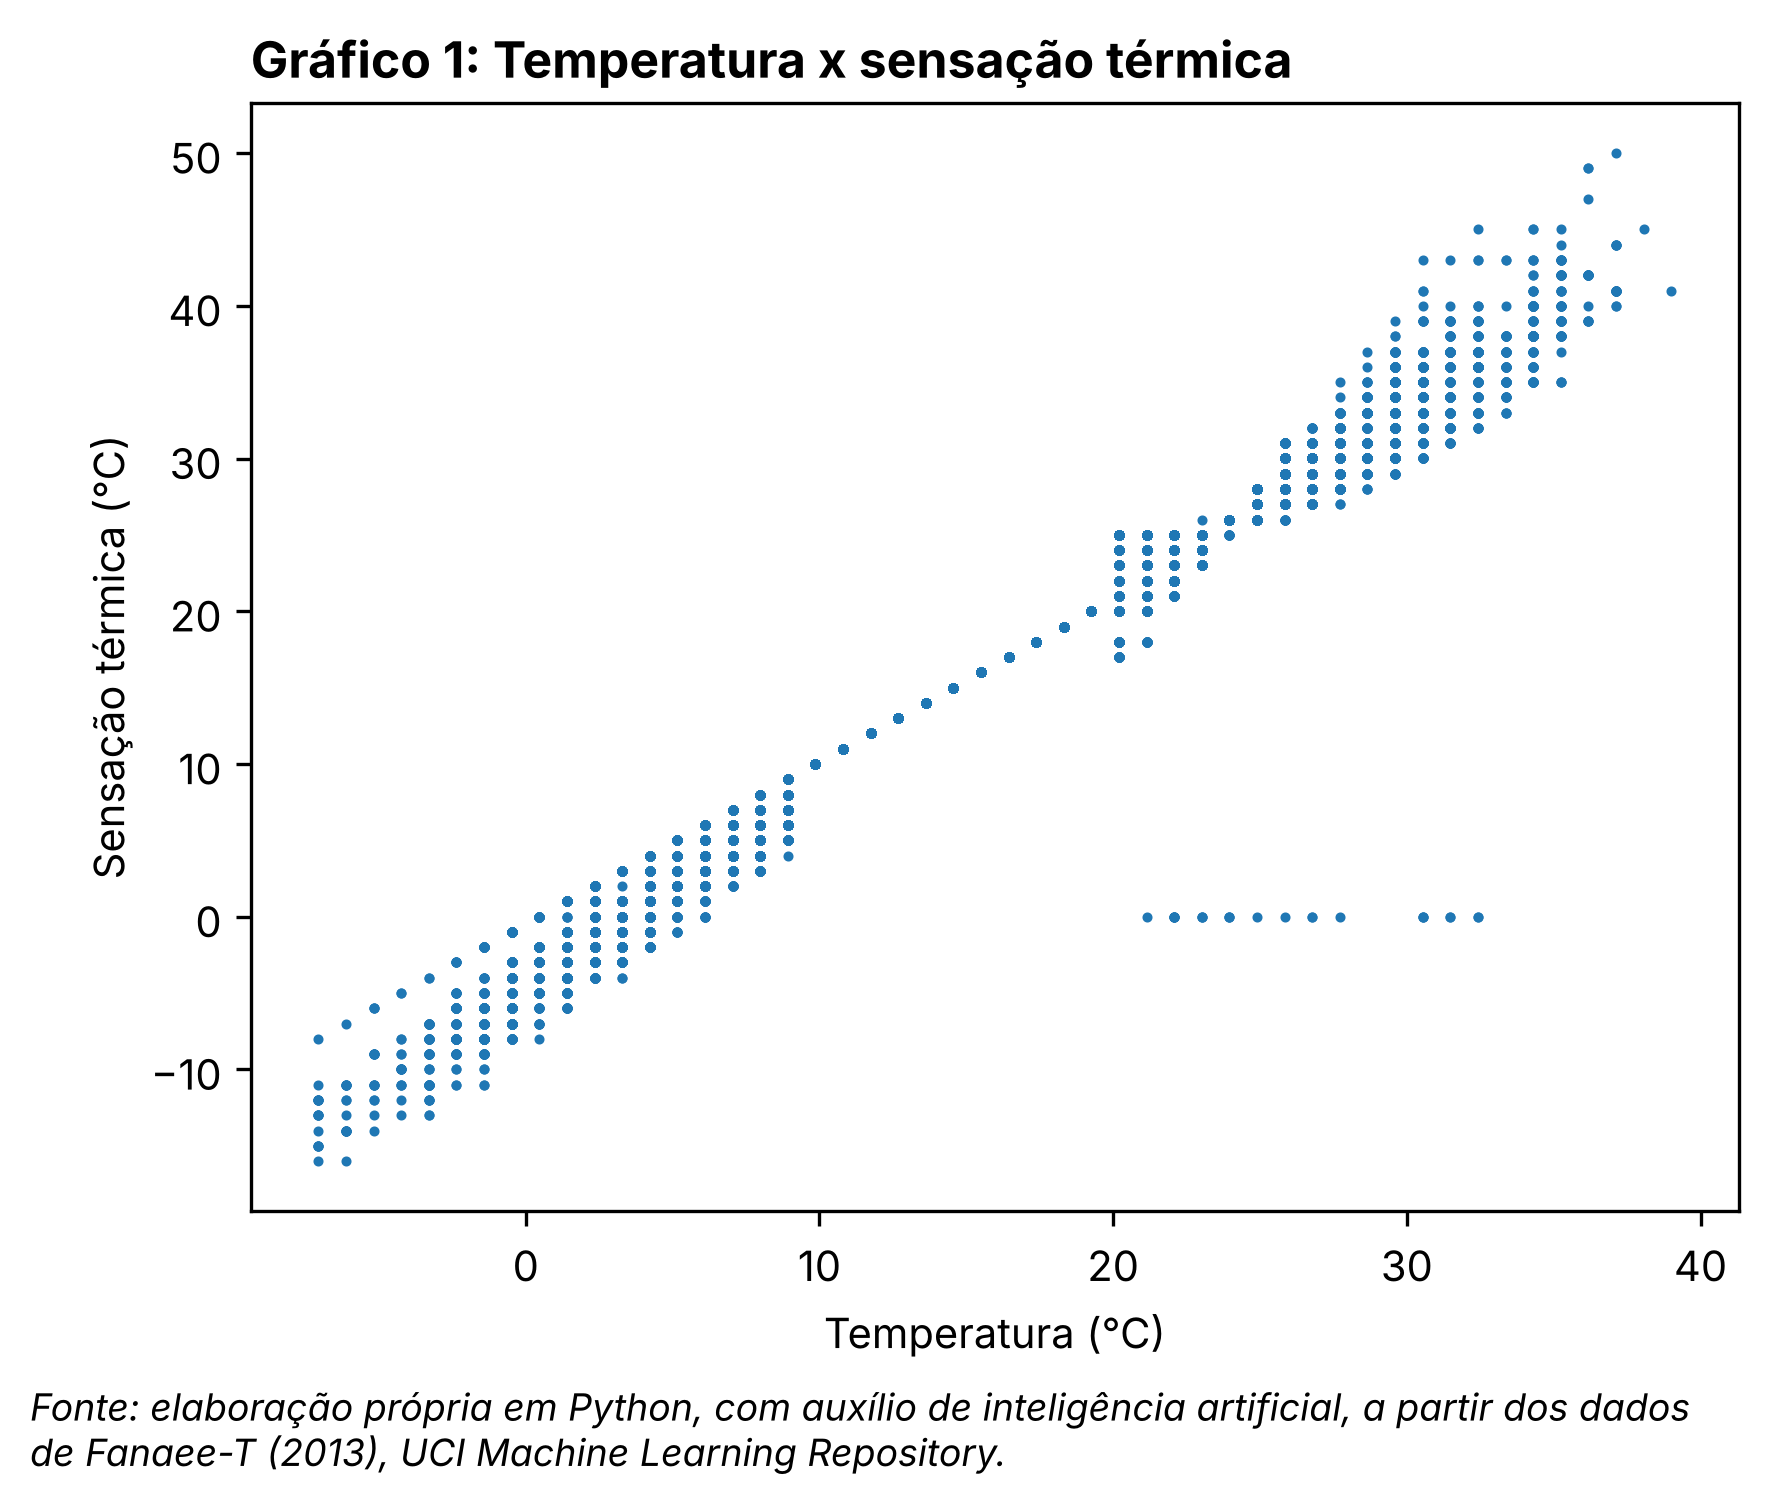
\includegraphics[width=0.72\linewidth,height=\textheight,keepaspectratio]{figuras/grafico_1.png}
		
	}
	
\end{figure}%

\clearpage

\section{Análise exploratória}\label{anuxe1lise-exploratuxf3ria}

Quatro perguntas orientaram a exploração, cada uma indicando variáveis
que deveriam pesar na previsão: \texttt{hr} e \texttt{yr},
\texttt{season}, \texttt{temp}, e \texttt{hr} junto com
\texttt{workingday}.

\subsection{Em que horas se aluga mais, e o padrão se mantém de 2011
para
2012?}\label{em-que-horas-se-aluga-mais-e-o-padruxe3o-se-mantuxe9m-de-2011-para-2012}

A demanda varia fortemente ao longo do dia, com dois picos, por volta
das 8h e das 17h--18h, e mínimo de madrugada (Gráfico 1). O
formato é o mesmo nos dois anos, mas a média horária passou de 143,8 em
2011 para 234,7 em 2012, alta de \textbf{63\%}. A razão entre as médias
de 2012 e 2011 fica entre 1,33 e 1,73 em todas as horas, o que indica um
crescimento generalizado, compatível com a expansão do sistema. Logo,
\texttt{hr} e \texttt{yr} devem ser importantes para prever
\texttt{cnt}.

\begin{figure}

\centering{

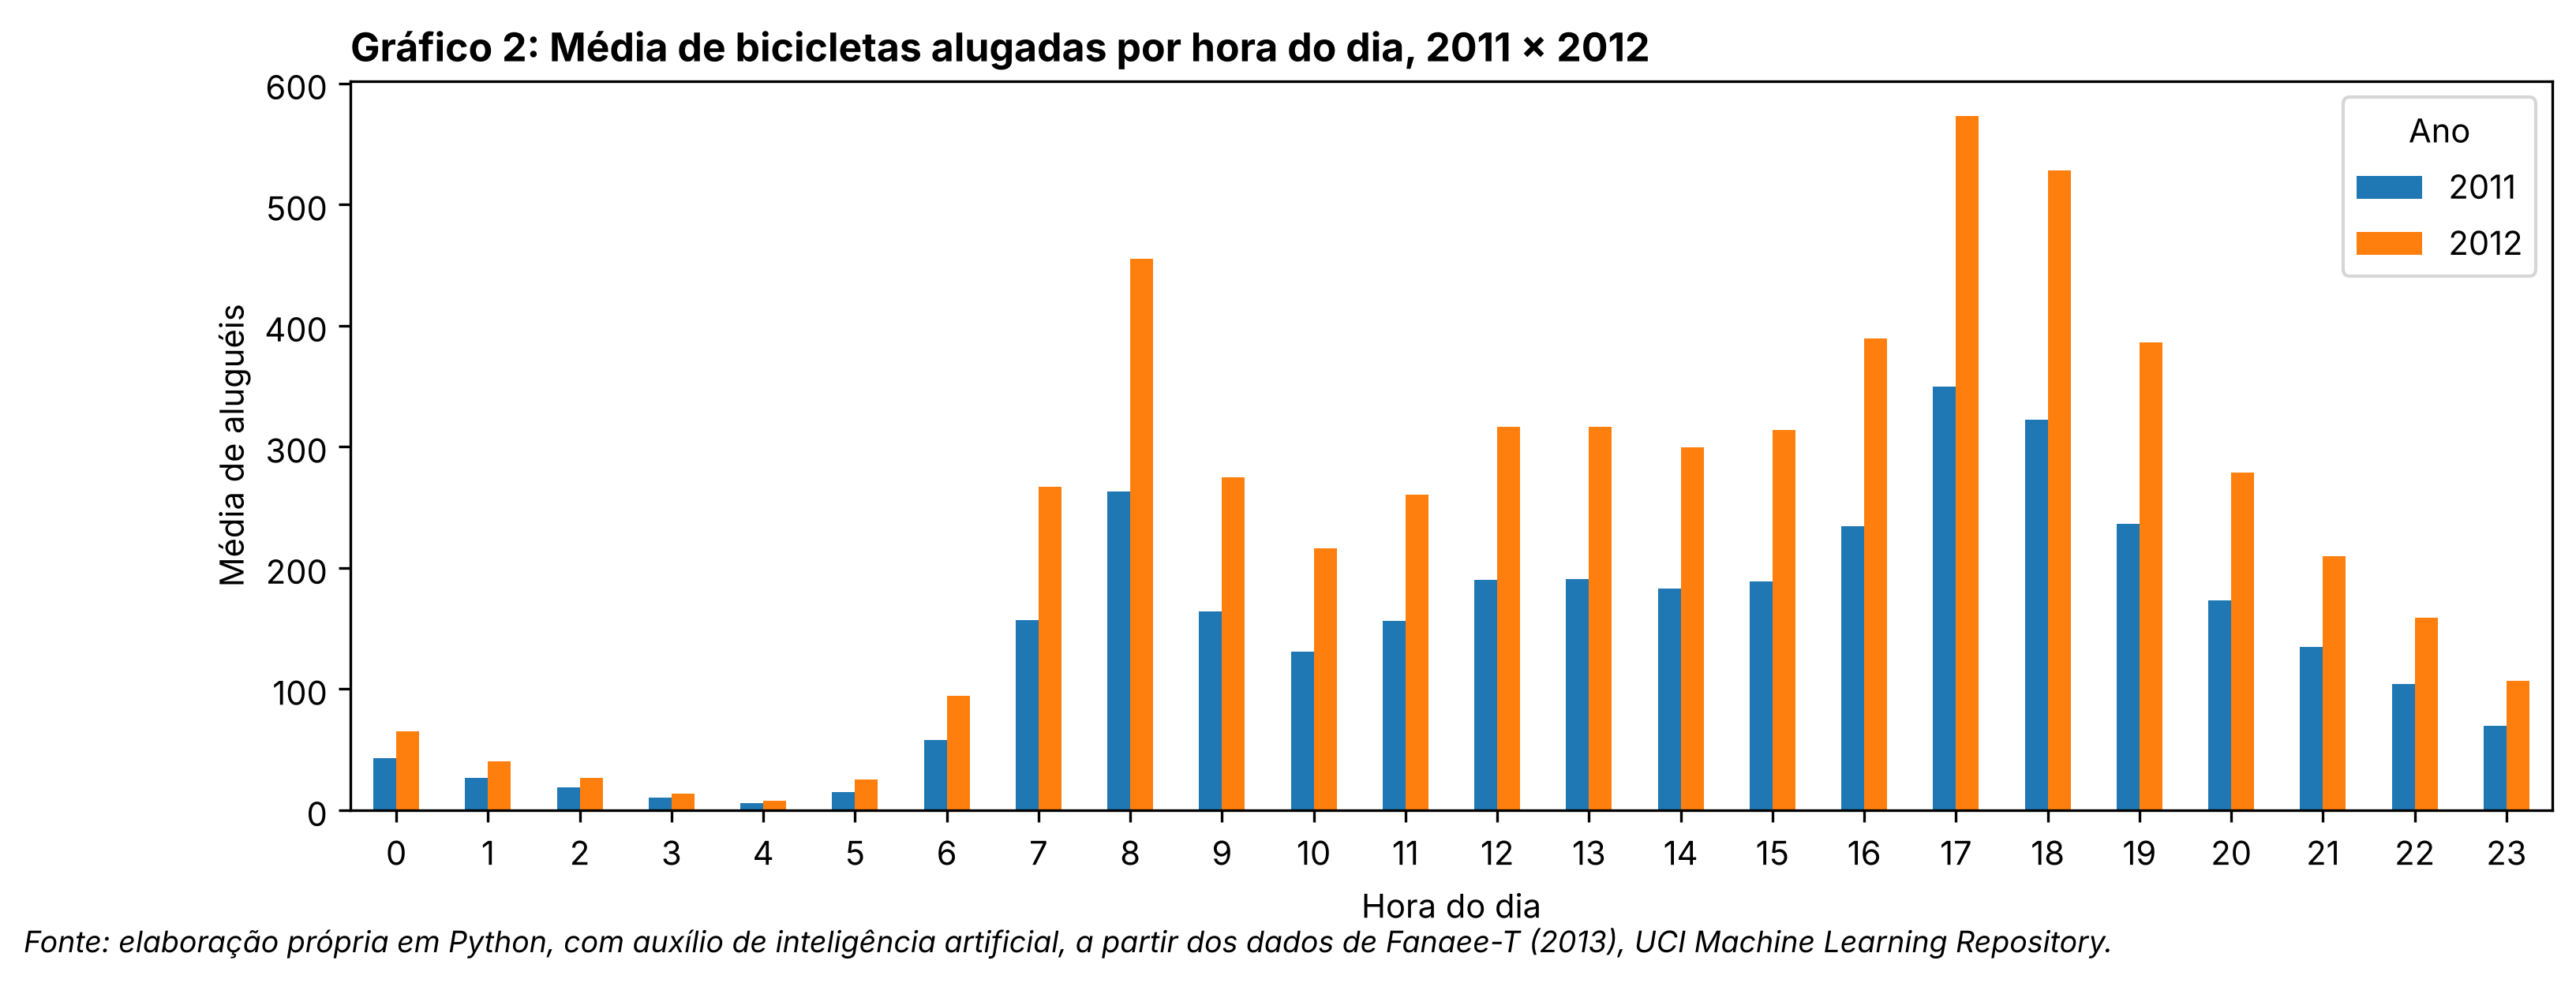
\includegraphics[width=0.85\linewidth,height=\textheight,keepaspectratio]{figuras/grafico_2.png}

}

\end{figure}%

\subsection{A demanda muda conforme a estação do
ano?}\label{a-demanda-muda-conforme-a-estauxe7uxe3o-do-ano}

Sim. A demanda é mais baixa no inverno e mais alta no verão, com
primavera e outono em posição intermediária, e o padrão se repete nos
dois anos (Gráfico 3 e Tabela~\ref{tbl-estacoes}). O
inverno teve o maior crescimento relativo entre os anos (112\%),
partindo de uma base baixa. Aparecem também quedas pontuais ligadas a
eventos, como o furacão Sandy no outono de 2012.

\begin{figure}

\centering{

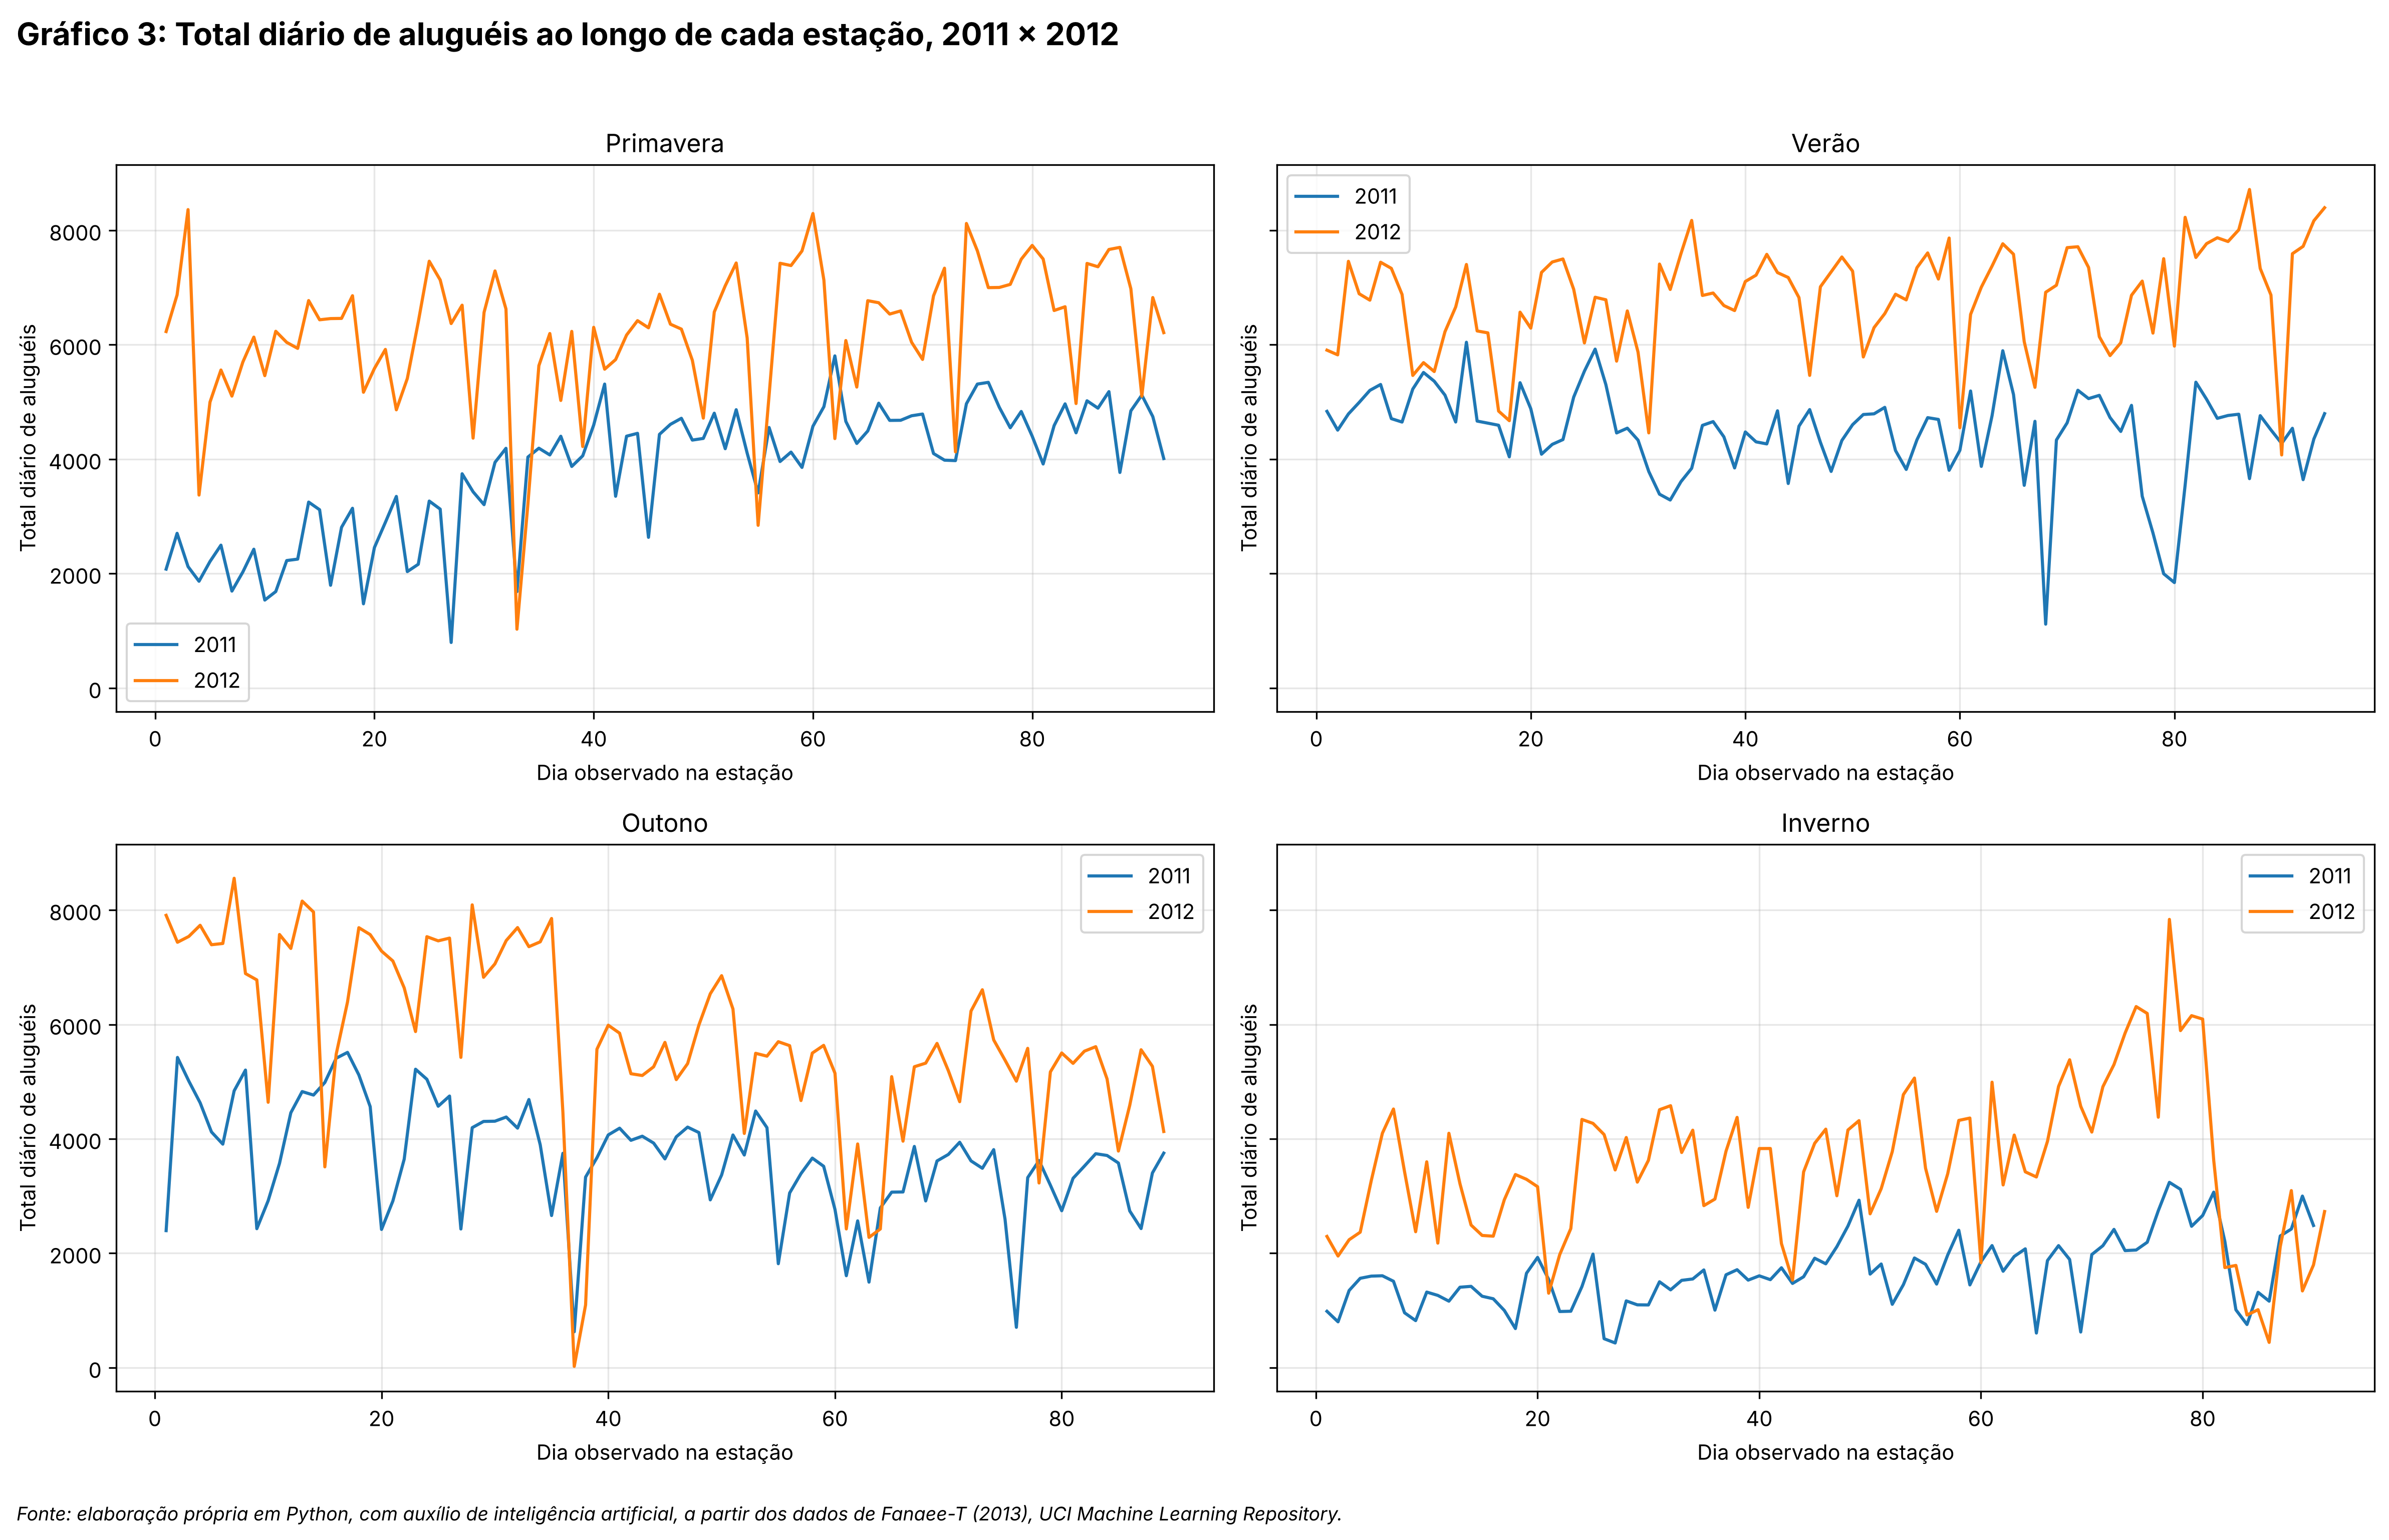
\includegraphics[width=1.0\linewidth,height=\textheight,keepaspectratio]{figuras/grafico_3.png}

}


\end{figure}%

{\setlength{\LTpost}{0pt}
	\begin{longtable}[]{@{}lrrr@{}}
		\toprule\noalign{}
		Estação & 2011 & 2012 & Variação (\%) \\
		\midrule\noalign{}
		\endfirsthead
		\toprule\noalign{}
		Estação & 2011 & 2012 & Variação (\%) \\
		\midrule\noalign{}
		\endhead
		\bottomrule\noalign{\vskip 4pt}
		\caption{Média do total diário de aluguéis por estação e ano
			(2011--2012), com variação percentual entre os anos.}\label{tbl-estacoes}\\[-8pt]
		\endlastfoot
		Inverno & 1.667 & 3.531 & 112\% \\
		Primavera & 3.775 & 6.209 & 64\% \\
		Verão & 4.464 & 6.824 & 53\% \\
		Outono & 3.664 & 5.792 & 58\% \\
\end{longtable}}
{\centering\footnotesize Fonte: elaboração própria em Python, com auxílio de inteligência artificial, a partir dos dados de Fanaee-T (2013).\par}

\subsection{Dias quentes têm mais
aluguéis?}\label{dias-quentes-tuxeam-mais-aluguuxe9is}

Até certo ponto. A demanda cresce com a temperatura até uma faixa de
conforto, entre aproximadamente 20 e 30 °C, e diminui nos dias mais
quentes (Gráfico 4 e Tabela~\ref{tbl-tempfaixa}). Em 2012
nenhum dia teve média abaixo de -5 °C, e a queda acima de 30 °C se
baseia em apenas 12 dias, o que pede cautela. De todo modo, a relação
\textbf{não é linear}, o que favorece modelos baseados em árvores,
capazes de capturar efeitos diferentes em cada faixa de
temperatura.

\begin{figure}

\centering{

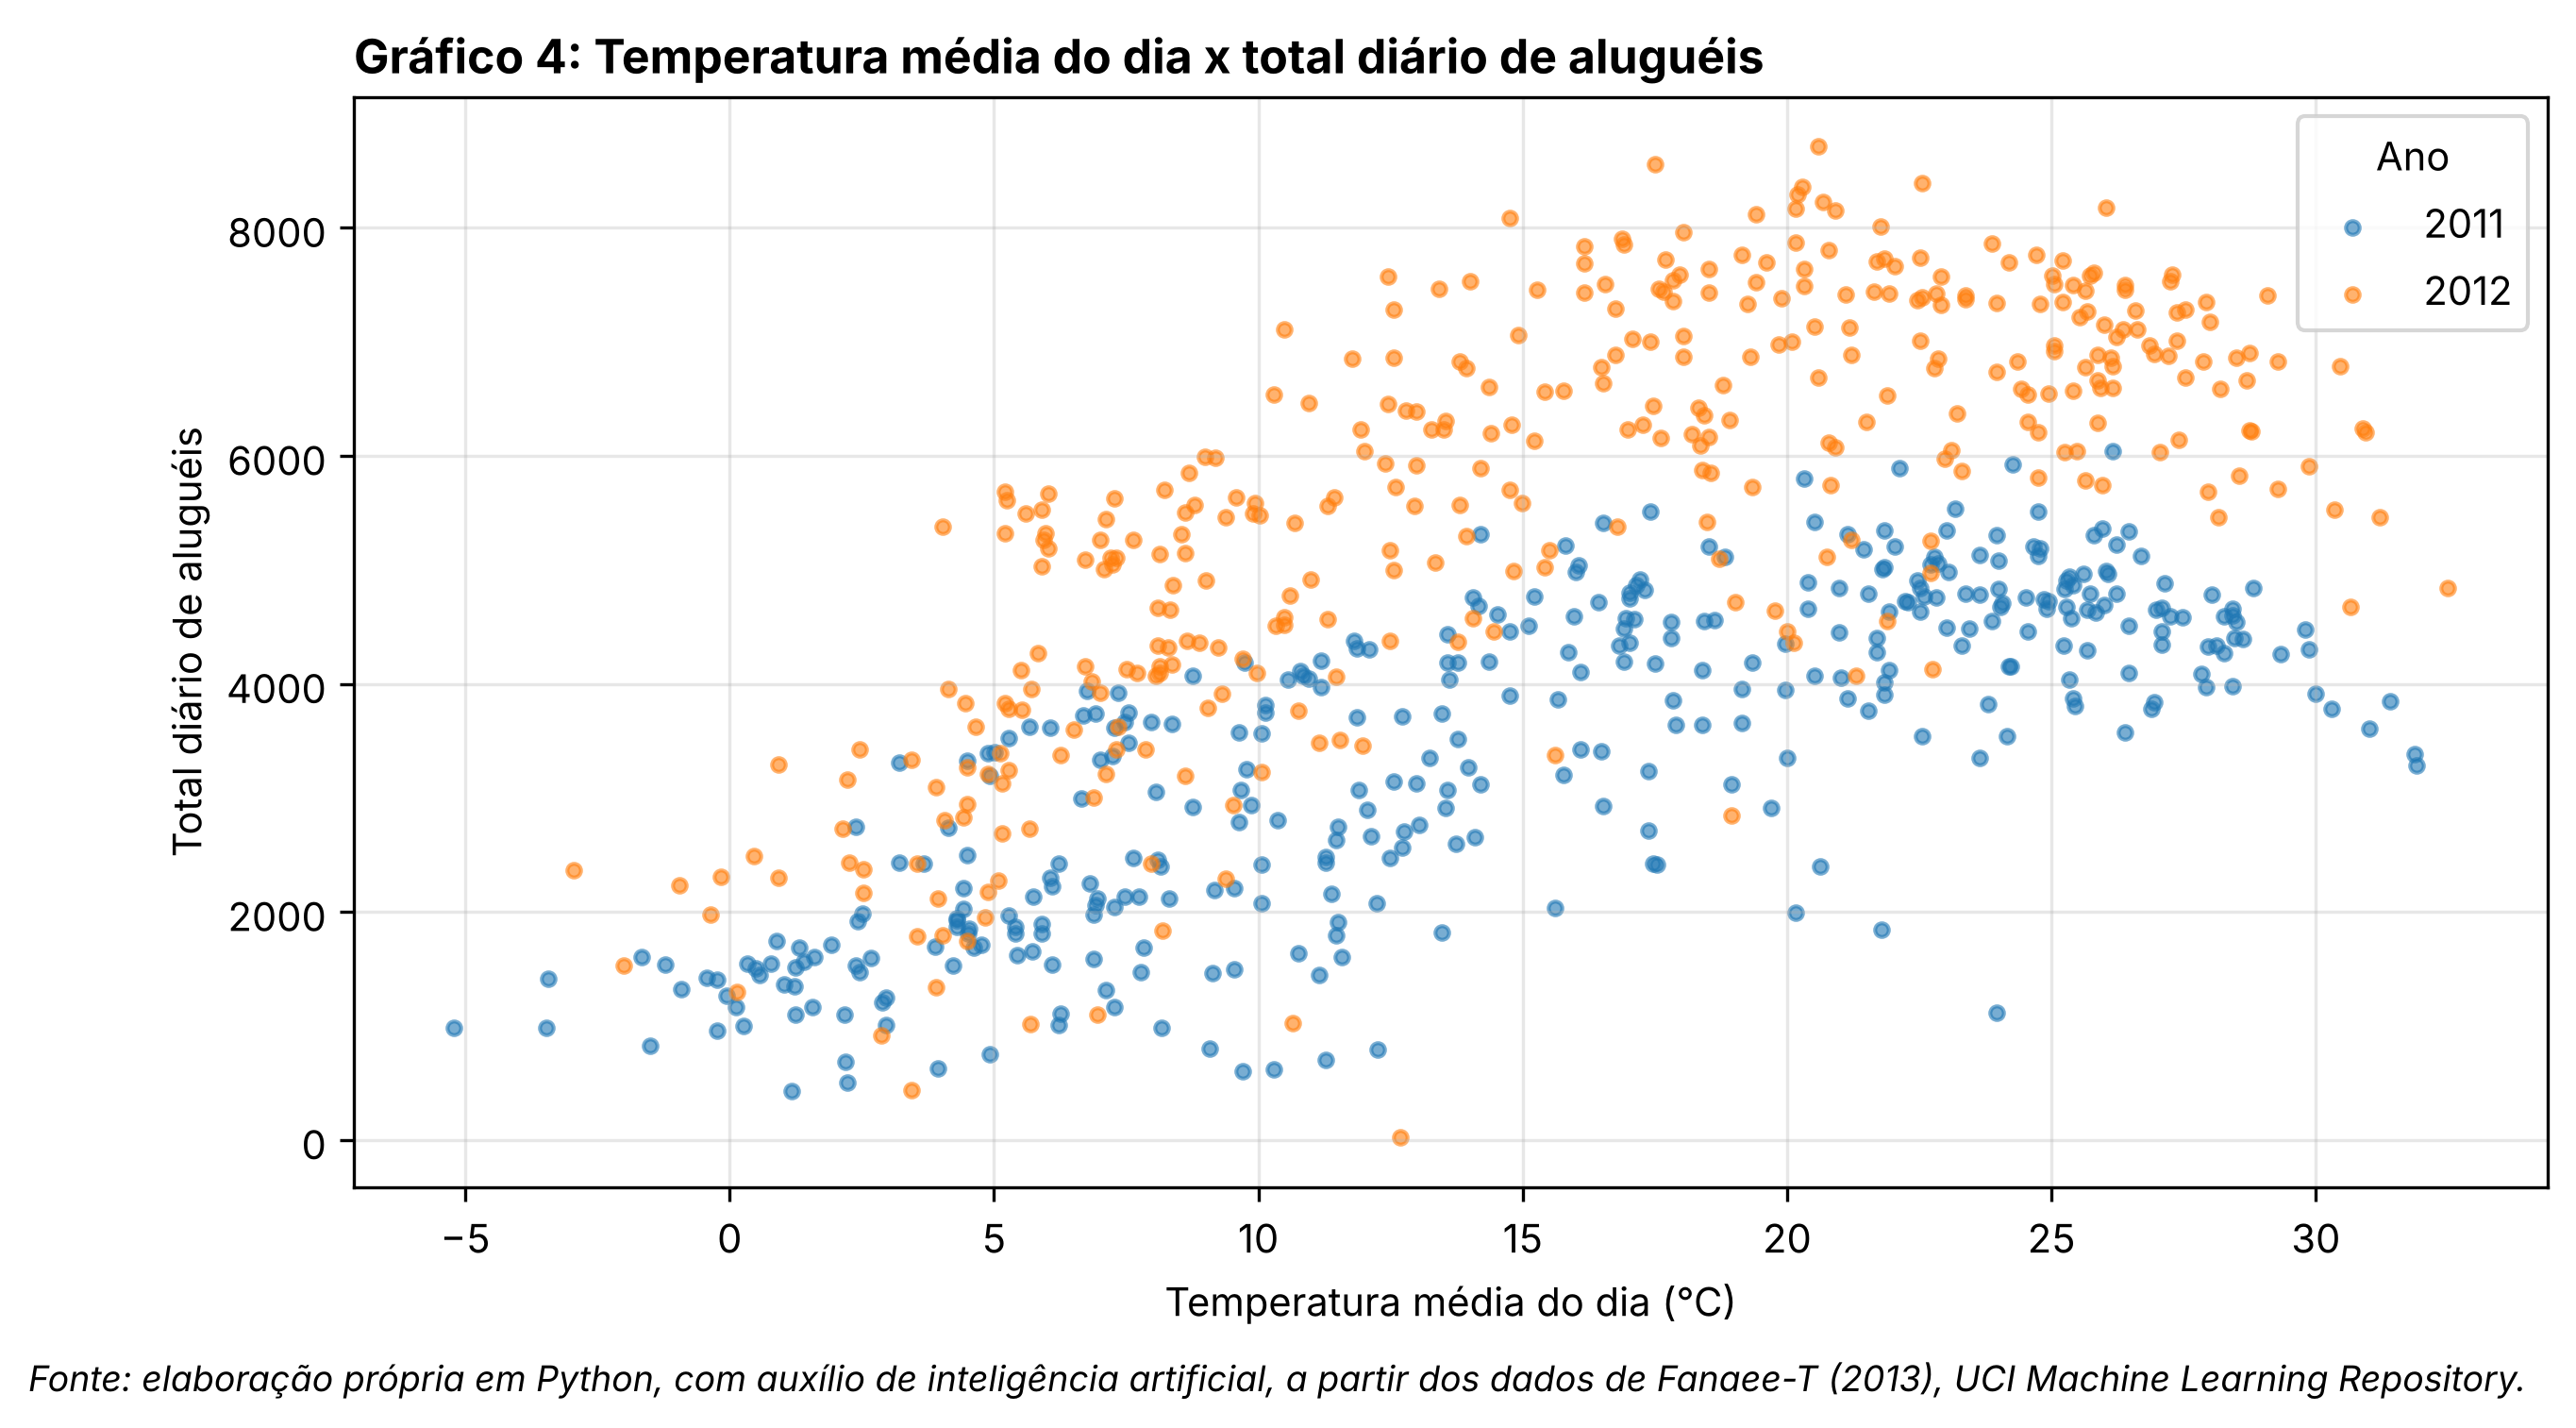
\includegraphics[width=0.83\linewidth,height=\textheight,keepaspectratio]{figuras/grafico_4.png}

}
\end{figure}%

{\setlength{\LTpost}{0pt}
	\begin{longtable}[]{@{}
			>{\raggedright\arraybackslash}p{(\linewidth - 18\tabcolsep) * \real{0.2200}}
			>{\raggedleft\arraybackslash}p{(\linewidth - 18\tabcolsep) * \real{0.0867}}
			>{\raggedleft\arraybackslash}p{(\linewidth - 18\tabcolsep) * \real{0.0867}}
			>{\raggedleft\arraybackslash}p{(\linewidth - 18\tabcolsep) * \real{0.0867}}
			>{\raggedleft\arraybackslash}p{(\linewidth - 18\tabcolsep) * \real{0.0867}}
			>{\raggedleft\arraybackslash}p{(\linewidth - 18\tabcolsep) * \real{0.0867}}
			>{\raggedleft\arraybackslash}p{(\linewidth - 18\tabcolsep) * \real{0.0867}}
			>{\raggedleft\arraybackslash}p{(\linewidth - 18\tabcolsep) * \real{0.0867}}
			>{\raggedleft\arraybackslash}p{(\linewidth - 18\tabcolsep) * \real{0.0867}}
			>{\raggedleft\arraybackslash}p{(\linewidth - 18\tabcolsep) * \real{0.0867}}@{}}
		\toprule\noalign{}
		\begin{minipage}[b]{\linewidth}\raggedright
			Temp. média do dia
		\end{minipage} & \begin{minipage}[b]{\linewidth}\raggedleft
			-10 a -5
		\end{minipage} & \begin{minipage}[b]{\linewidth}\raggedleft
			-5 a 0
		\end{minipage} & \begin{minipage}[b]{\linewidth}\raggedleft
			0 a 5
		\end{minipage} & \begin{minipage}[b]{\linewidth}\raggedleft
			5 a 10
		\end{minipage} & \begin{minipage}[b]{\linewidth}\raggedleft
			10 a 15
		\end{minipage} & \begin{minipage}[b]{\linewidth}\raggedleft
			15 a 20
		\end{minipage} & \begin{minipage}[b]{\linewidth}\raggedleft
			20 a 25
		\end{minipage} & \begin{minipage}[b]{\linewidth}\raggedleft
			25 a 30
		\end{minipage} & \begin{minipage}[b]{\linewidth}\raggedleft
			30 a 35
		\end{minipage} \\
		\midrule\noalign{}
		\endfirsthead
		\toprule\noalign{}
		\begin{minipage}[b]{\linewidth}\raggedright
			Temp. média do dia
		\end{minipage} & \begin{minipage}[b]{\linewidth}\raggedleft
			-10 a -5
		\end{minipage} & \begin{minipage}[b]{\linewidth}\raggedleft
			-5 a 0
		\end{minipage} & \begin{minipage}[b]{\linewidth}\raggedleft
			0 a 5
		\end{minipage} & \begin{minipage}[b]{\linewidth}\raggedleft
			5 a 10
		\end{minipage} & \begin{minipage}[b]{\linewidth}\raggedleft
			10 a 15
		\end{minipage} & \begin{minipage}[b]{\linewidth}\raggedleft
			15 a 20
		\end{minipage} & \begin{minipage}[b]{\linewidth}\raggedleft
			20 a 25
		\end{minipage} & \begin{minipage}[b]{\linewidth}\raggedleft
			25 a 30
		\end{minipage} & \begin{minipage}[b]{\linewidth}\raggedleft
			30 a 35
		\end{minipage} \\
		\midrule\noalign{}
		\endhead
		\bottomrule\noalign{\vskip 4pt}
		\caption{Média do total diário de aluguéis por faixa de temperatura (°C)
			e ano (2011--2012).}\label{tbl-tempfaixa}\\[-8pt]
		\endlastfoot
		Média diária 2011 & 981 & 1.274 & 1.707 & 2.498 & 3.157 & 4.133 & 4.562
		& 4.558 & 3.582 \\
		Média diária 2012 & -- & 2.084 & 2.602 & 4.334 & 5.482 & 6.666 & 6.836 &
		6.850 & 5.677 \\
		Nº de dias & 1 & 15 & 81 & 143 & 120 & 110 & 134 & 115 & 12 \\
\end{longtable}}
{\centering\footnotesize Fonte: elaboração própria em Python, com auxílio de inteligência artificial, a partir dos dados de Fanaee-T (2013).\par}

\clearpage

\subsection{O padrão de uso é diferente em dias úteis e fins de
semana?}\label{o-padruxe3o-de-uso-uxe9-diferente-em-dias-uxfateis-e-fins-de-semana}

É diferente na distribuição ao longo do dia, mas não no volume
(Gráfico 5). Em dias úteis há dois picos, às 8h (477
aluguéis em média) e às 17h (525), compatíveis com o deslocamento
casa--trabalho. Em fins de semana e feriados a demanda se concentra
entre 12h e 17h, com pico às 13h (373), sugerindo uso para lazer e
passeio. O total diário médio é semelhante (4.585 em dias úteis contra
4.330, diferença de 5,9\%), e à meia-noite o fim de semana tem 2,5 vezes
mais aluguéis (91 contra 37). Como o efeito da hora depende do tipo de
dia, \texttt{hr} e \texttt{workingday} devem ser usadas em conjunto, e
árvores conseguem capturar essa interação.

\begin{figure}

\centering{

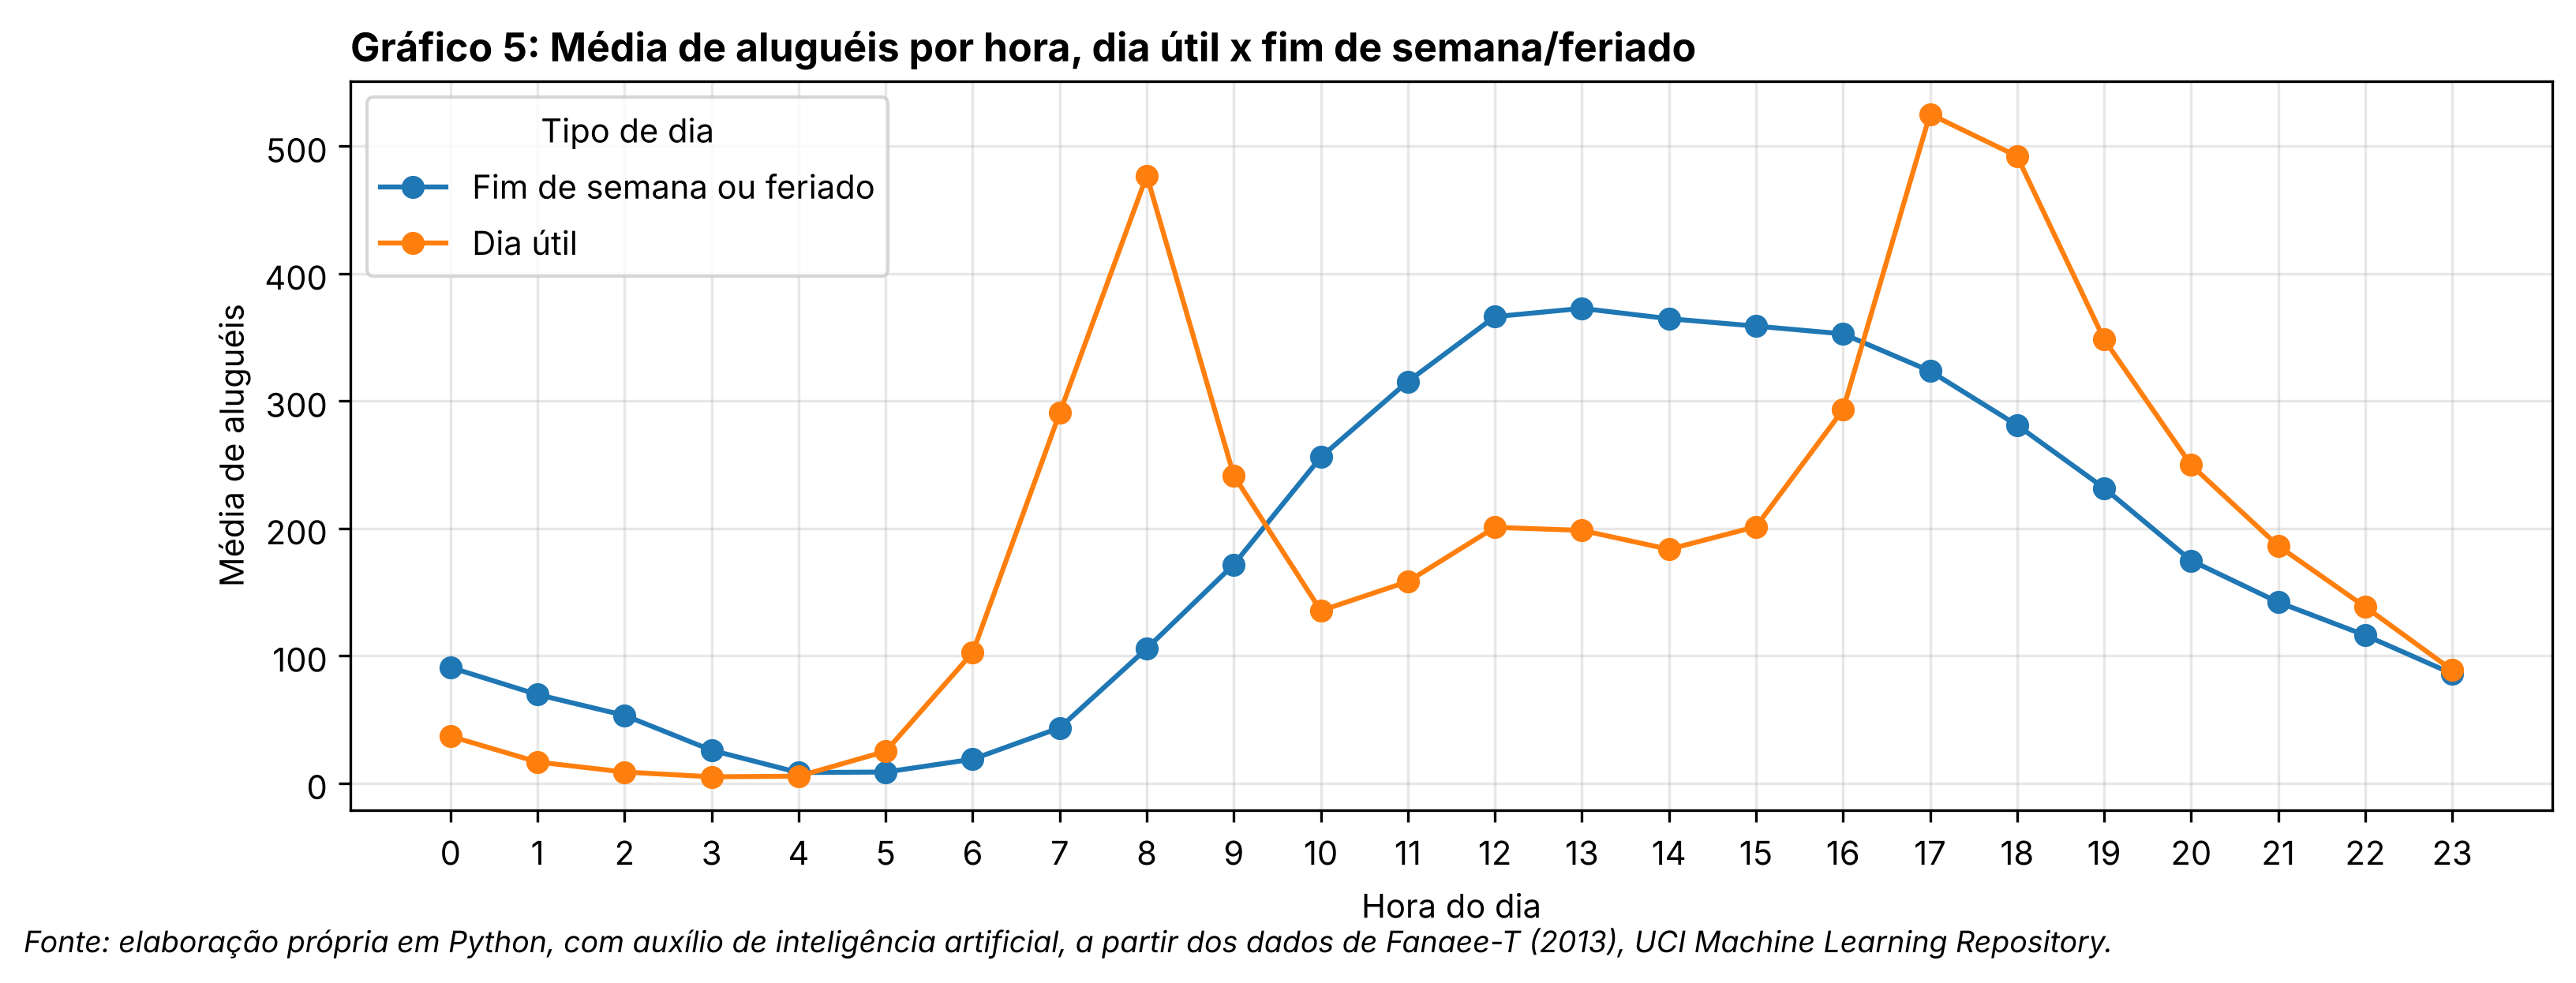
\includegraphics[width=0.85\linewidth,height=\textheight,keepaspectratio]{figuras/grafico_5.png}

}

\end{figure}%


\section{Modelagem e resultados}\label{modelagem-e-resultados}

\subsection{Linha de base}\label{linha-de-base}

Com base na análise 4, a regra de referência prevê, para cada hora do
teste, a média de \texttt{cnt} daquela mesma hora e do mesmo tipo de dia
(útil ou não) no período de treino. Ela obteve MAE = 80,0, RMSE = 119,6
e R² = 0,648: erra em média 80 bicicletas por hora e explica cerca de
65\% da variação, bem acima de ``chutar a média'' (R² = 0), mas deixa
35\% sem explicação. A regra não conhece clima, temperatura, estação nem
ano, e como mistura 2011 e 2012, tende a subestimar o fim de 2012 (a
linha tracejada do Gráfico 7).

\begin{figure}
	
	\centering{
		
		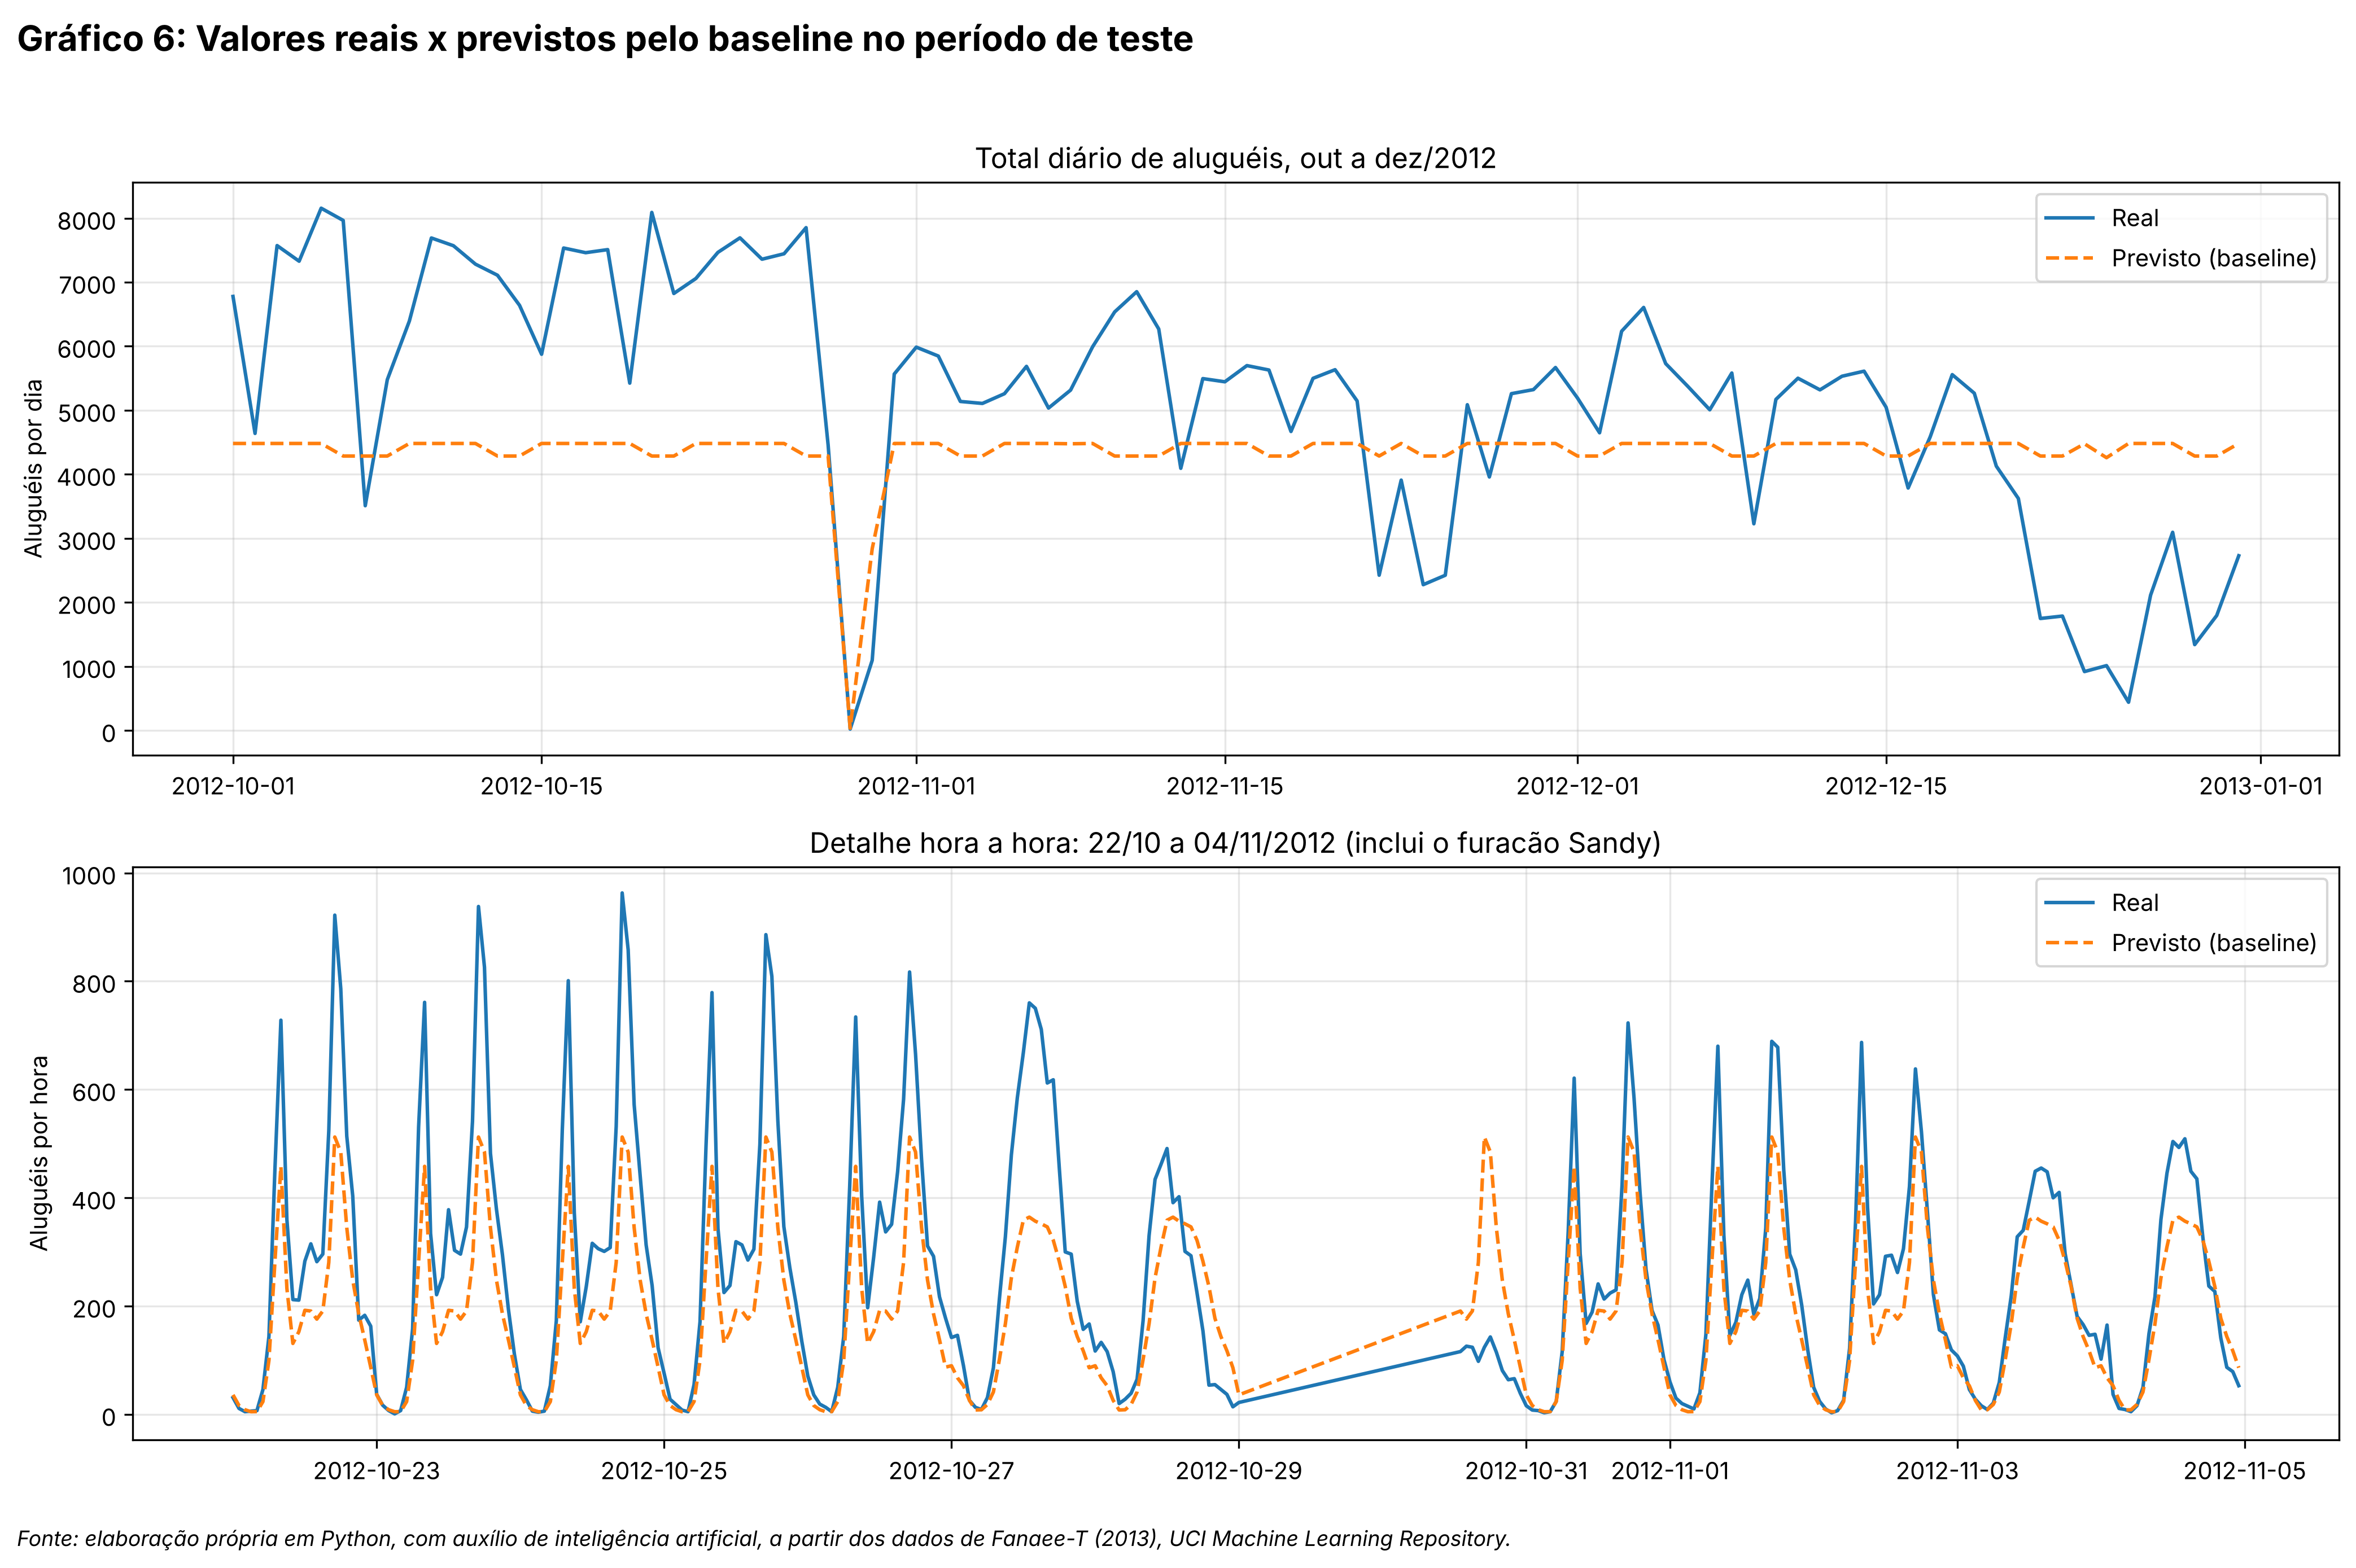
\includegraphics[width=0.85\linewidth,height=\textheight,keepaspectratio]{figuras/grafico_6.png}
		
	}
	
\end{figure}%
	
\end{figure}%

\clearpage

\subsection{Árvore de decisão}\label{uxe1rvore-de-decisuxe3o}

Uma árvore sem limite de crescimento (profundidade 30 e 14.428 folhas)
decorou o treino, com MAE = 0,0 e R² = 1,000, contra MAE = 56,8 e R² =
0,809 no teste, um claro sinal de sobreajuste. Para corrigir isso,
testaram-se profundidades máximas de 2 a 20, além de ``sem limite'',
usando o erro na validação (jul a set/2012). O erro de validação cai até
a profundidade 10 (MAE = 50,5) e se estabiliza depois, enquanto o erro
de treino segue caindo até zero (Gráfico7 e
Tabela~\ref{tbl-prof}). Foi escolhida a profundidade 10, a mais simples
entre as de desempenho equivalente.

\begin{figure}

\centering{

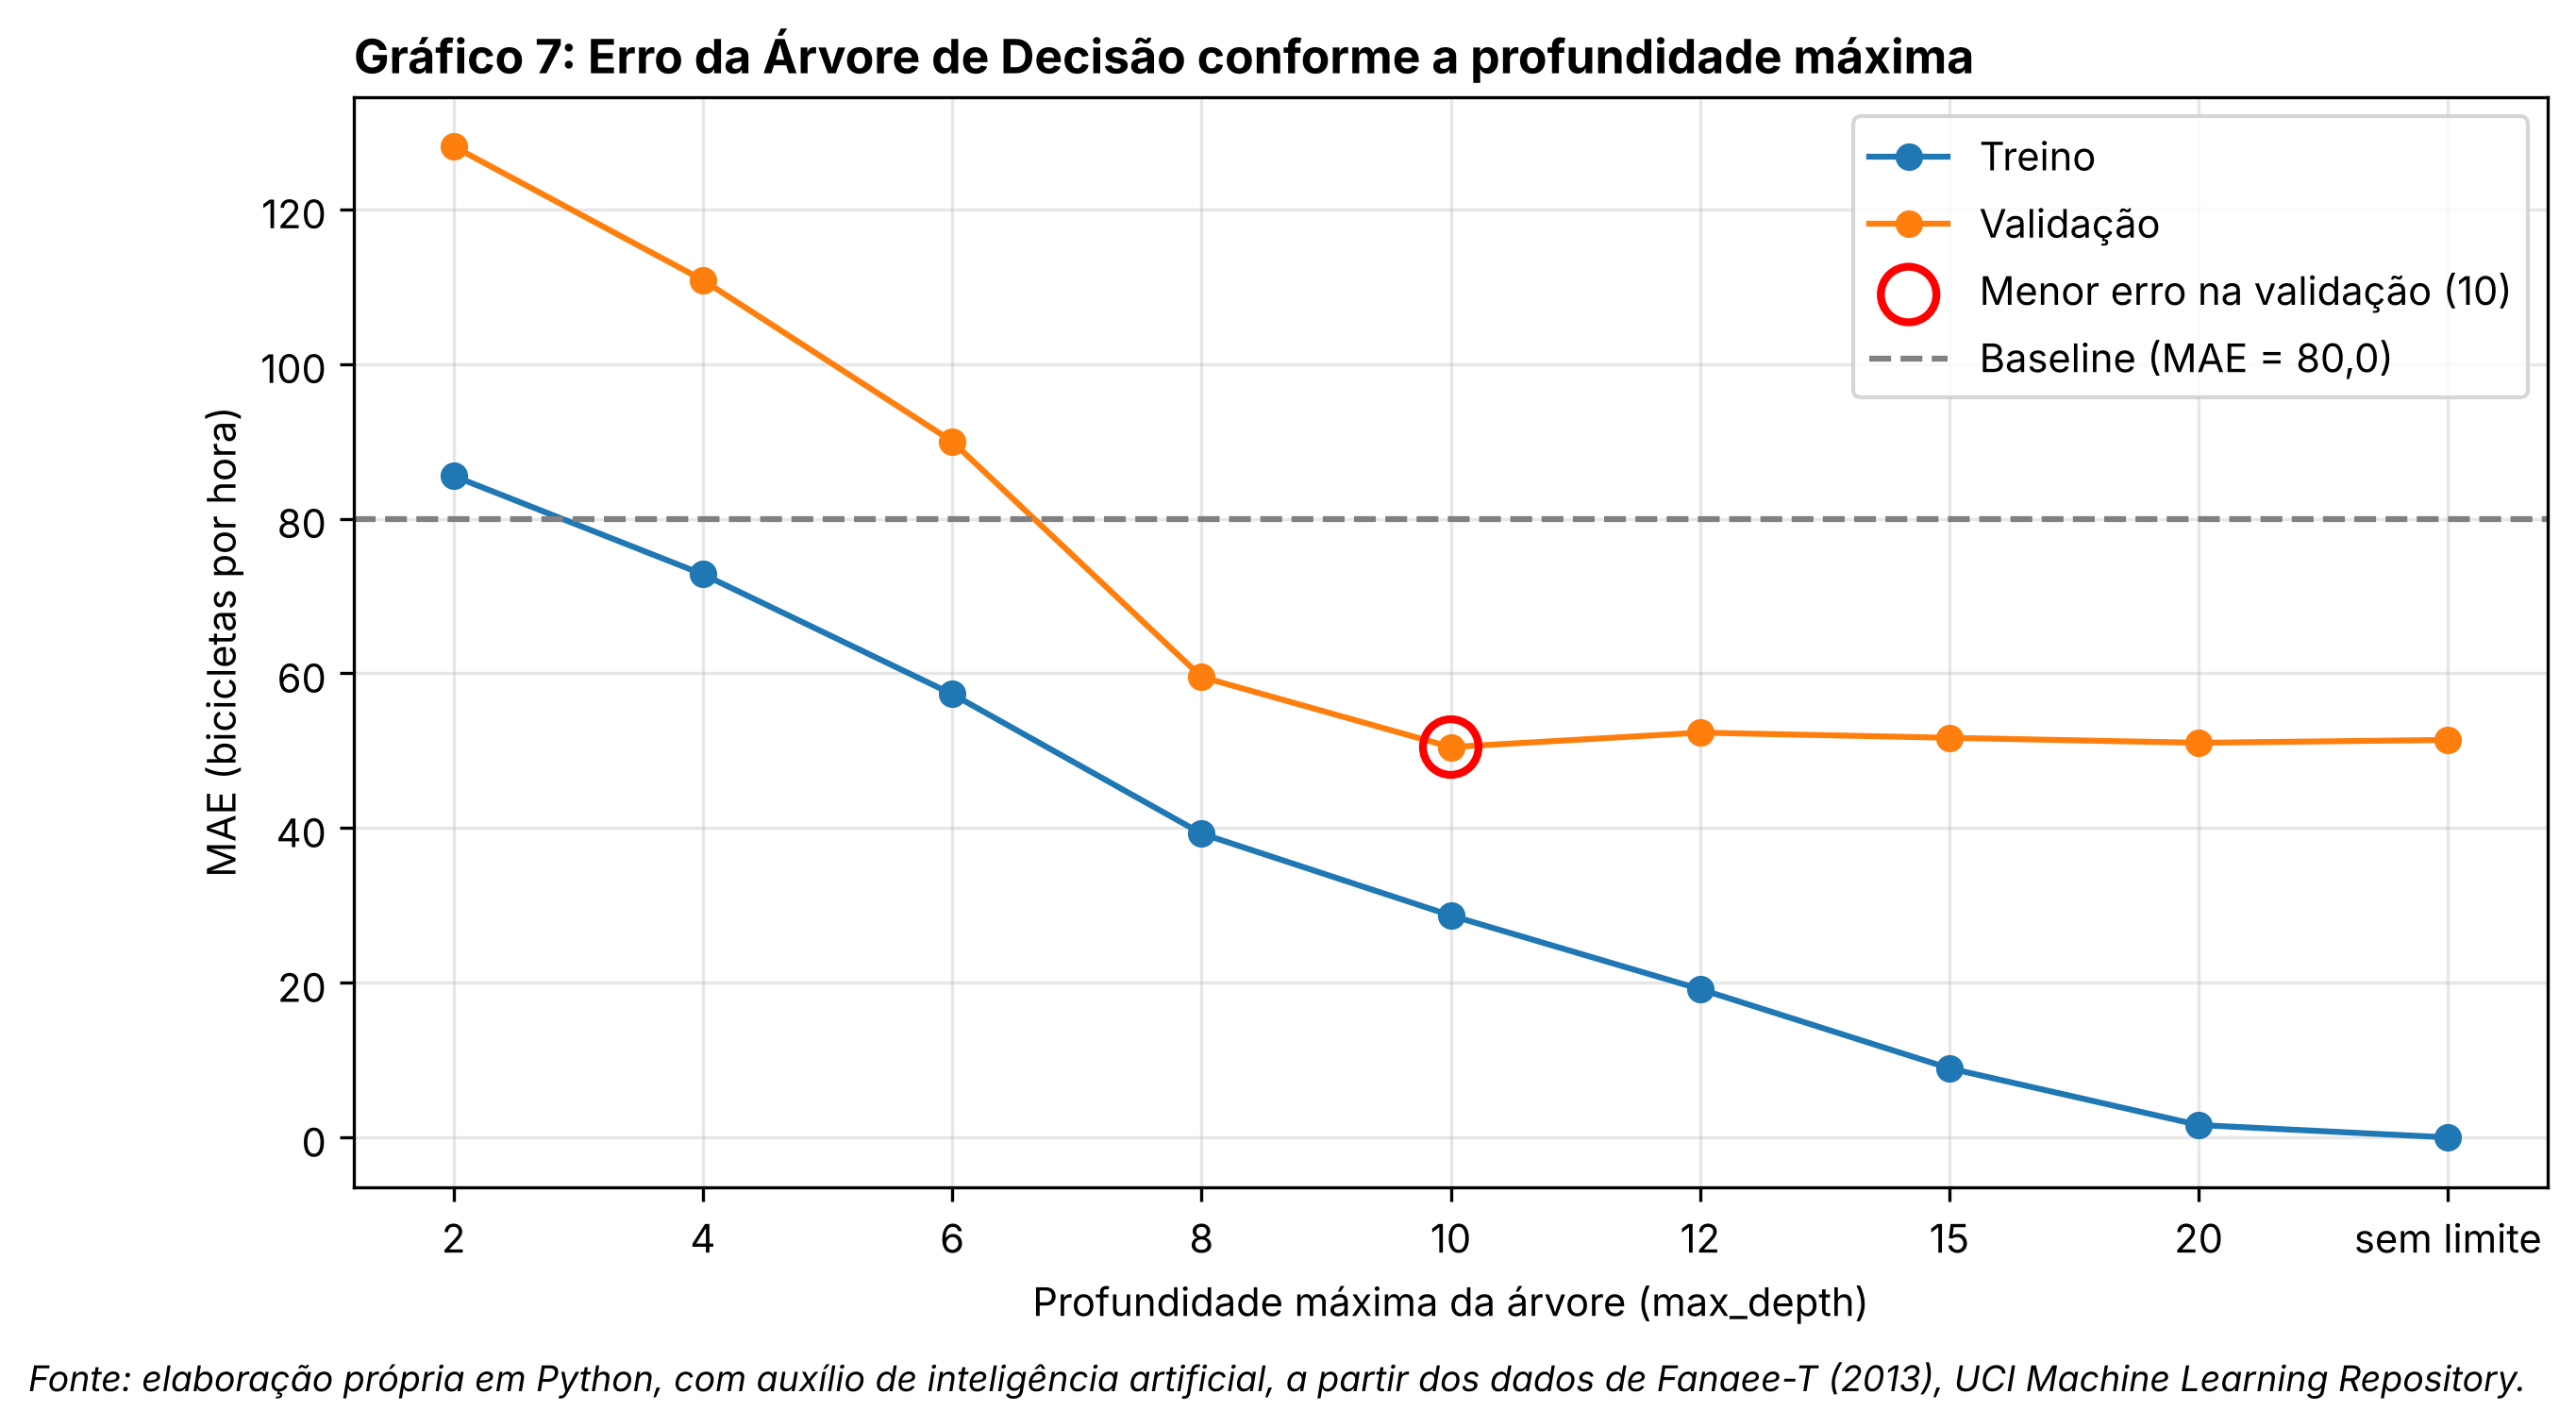
\includegraphics[width=0.75\linewidth,height=\textheight,keepaspectratio]{figuras/grafico_7.png}

}

\end{figure}%


{\setlength{\LTpost}{0pt}
	\begin{longtable}[]{@{}lrrrrr@{}}
		\toprule\noalign{}
		Profundidade & 10 & 12 & 15 & 20 & sem limite \\
		\midrule\noalign{}
		\endfirsthead
		\toprule\noalign{}
		Profundidade & 10 & 12 & 15 & 20 & sem limite \\
		\midrule\noalign{}
		\endhead
		\bottomrule\noalign{\vskip 4pt}
		\caption{Erro absoluto médio (MAE) da árvore de decisão na validação
			(jul a set/2012), por profundidade
			máxima.}\label{tbl-prof}\\[-8pt]
		\endlastfoot
		MAE na validação & 50,5 & 52,3 & 51,7 & 51,0 & 51,4 \\
\end{longtable}}
{\centering\footnotesize Fonte: elaboração própria em Python, com auxílio de inteligência artificial, a partir dos dados de Fanaee-T (2013).\par}


Reajustada com o treino completo, a árvore de profundidade 10 obteve no
teste MAE = 60,4, RMSE = 94,6 e R² = 0,780, ou seja, melhor que o
\emph{baseline}, mas pior que a árvore sem limite
(Gráfico 7). A diferença entre a melhor e a pior
profundidade na validação é de menos de 2 bicicletas (cerca de 4\%), o
que ilustra a instabilidade de uma árvore única: pequenas mudanças nos
dados mudam a primeira pergunta e, com ela, todas as perguntas abaixo.

\begin{figure}

\centering{

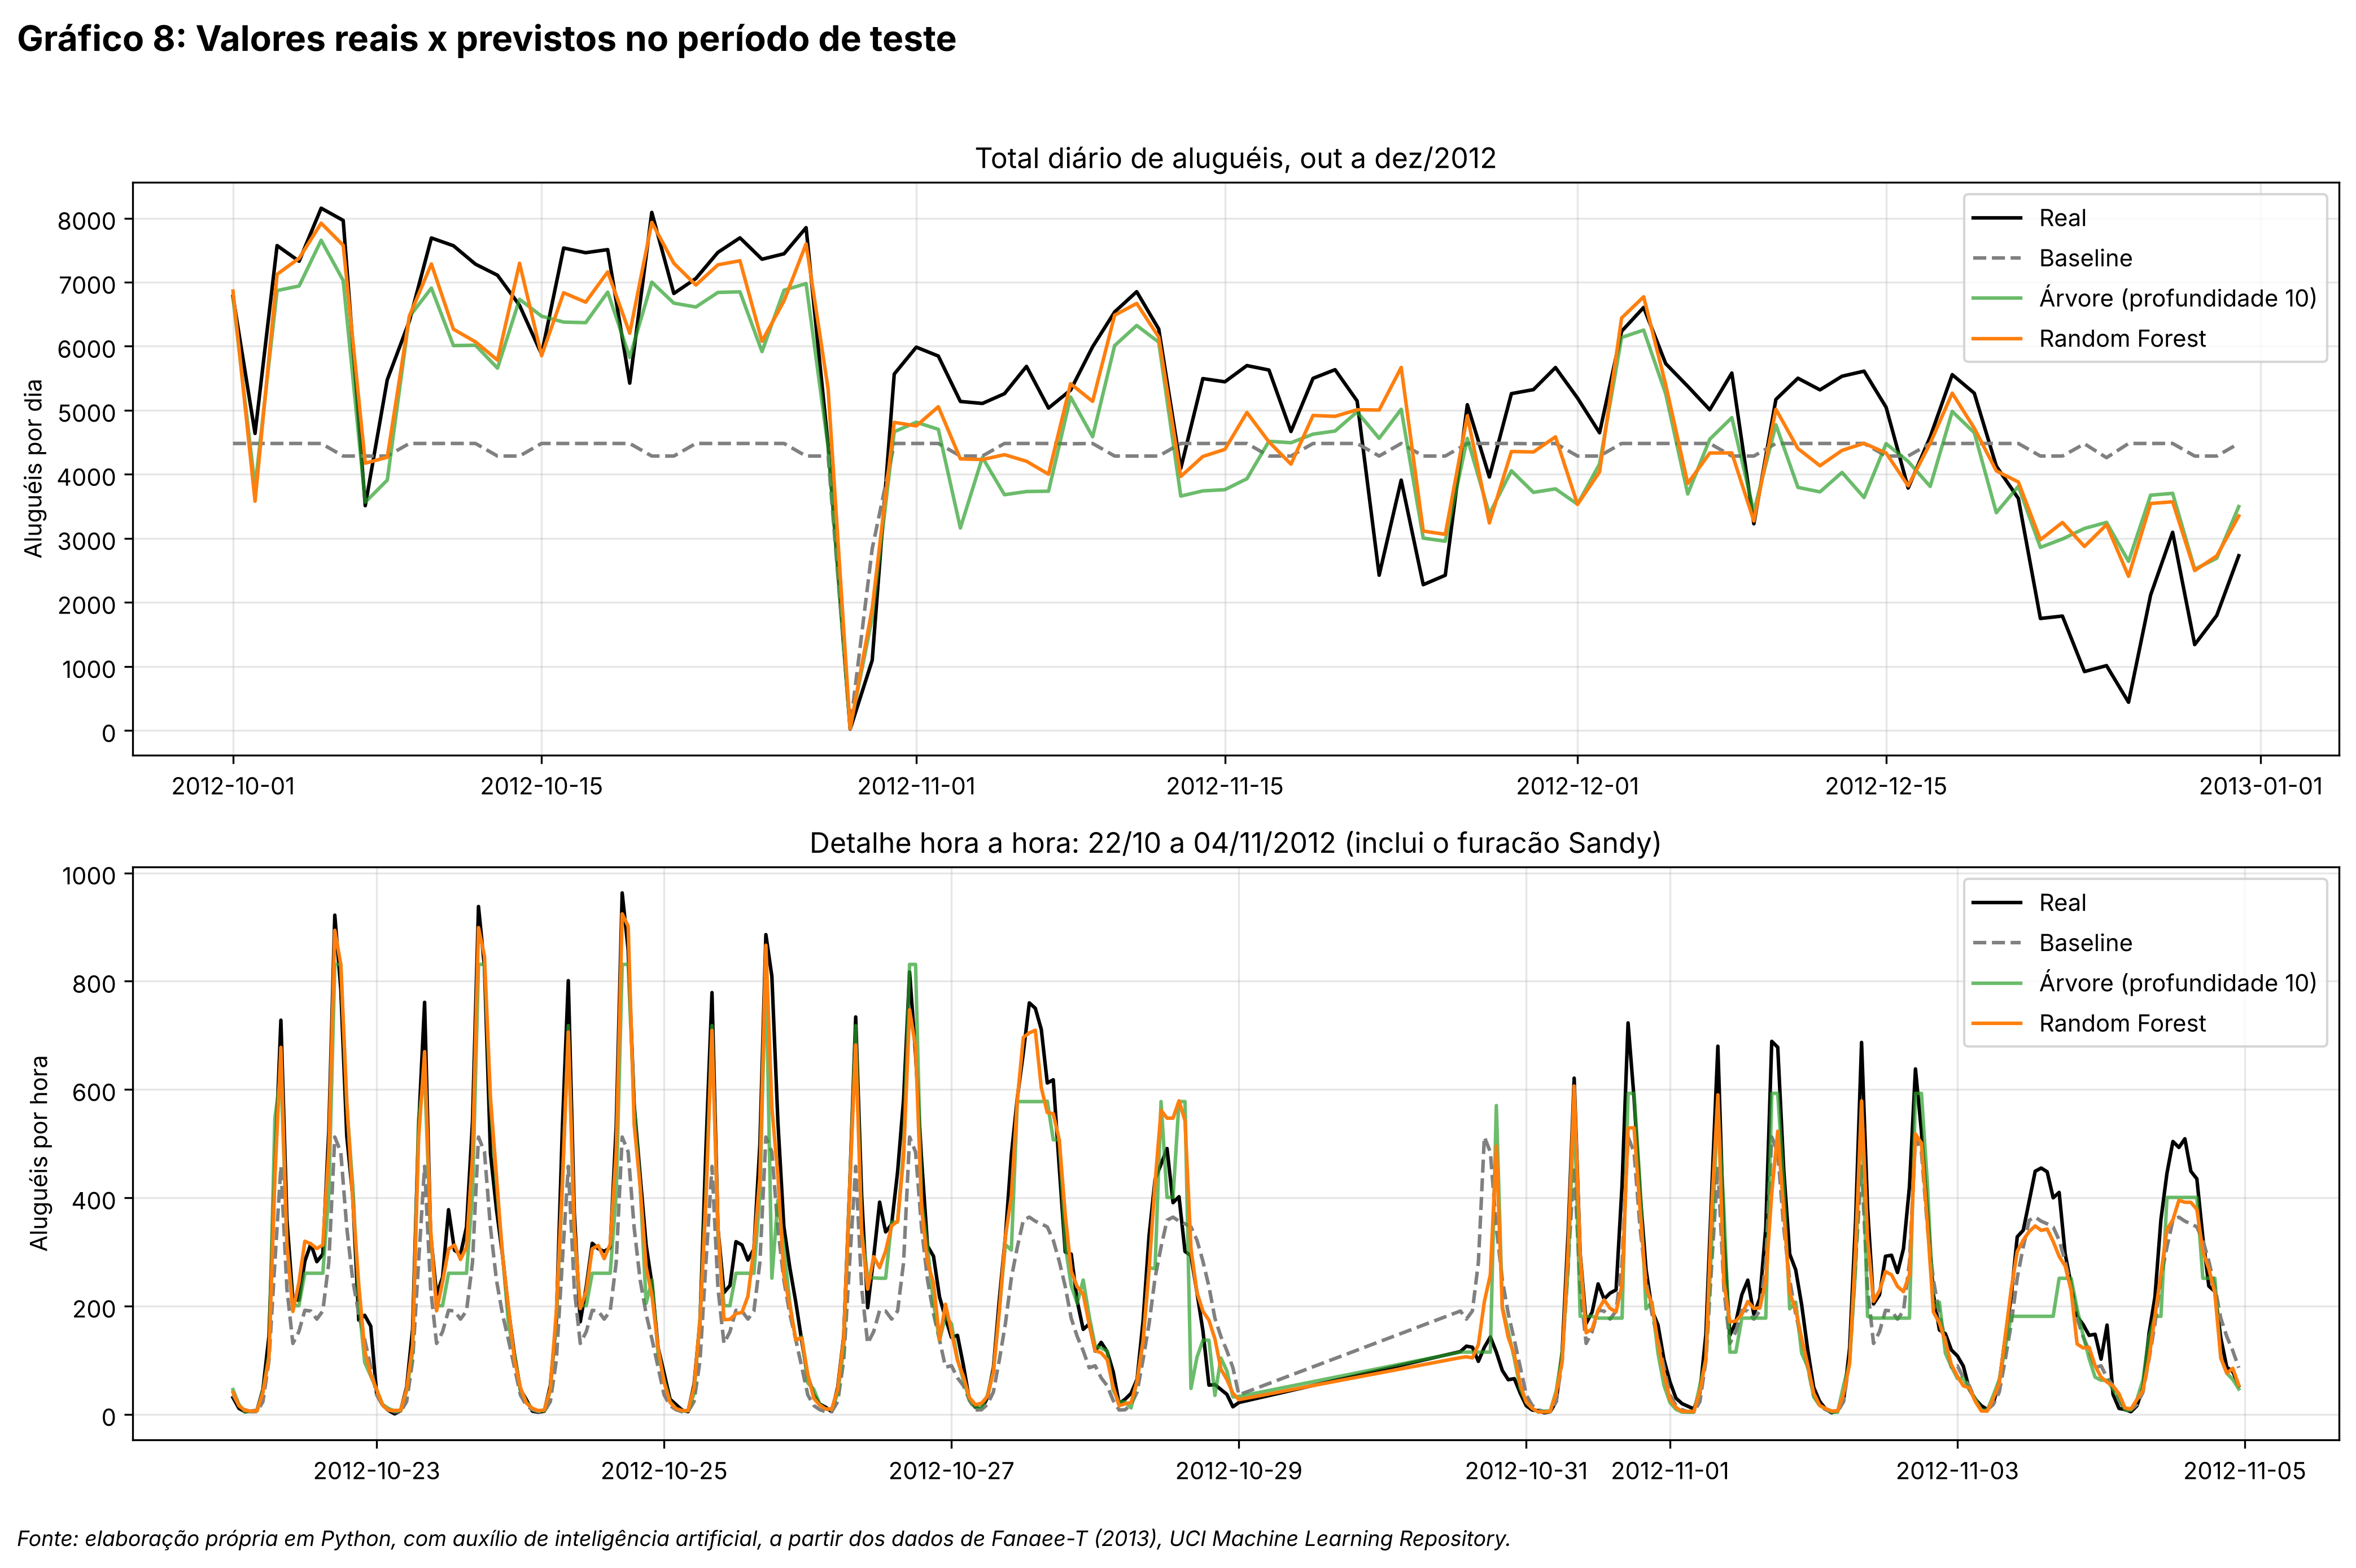
\includegraphics[width=0.85\linewidth,height=\textheight,keepaspectratio]{figuras/grafico_8.png}

}

\end{figure}%

\subsection{Floresta aleatória}\label{floresta-aleatuxf3ria}

Para reduzir essa instabilidade, ajustou-se uma floresta com 200 árvores
e demais parâmetros no padrão. No teste, obteve MAE = 46,9, RMSE = 72,0
e R² = 0,872 (treino: MAE = 8,8). Em média, a floresta erra 47
bicicletas por hora, contra 80 do \emph{baseline} (redução de cerca de
41\%) e 56,8 da melhor árvore (cerca de 17\% a menos). O RMSE também é o
menor, o que indica menos erros grandes.

\subsection{Comparação dos modelos}\label{comparauxe7uxe3o-dos-modelos}

{\setlength{\LTpost}{0pt}
	\begin{longtable}[]{@{}
			>{\raggedright\arraybackslash}p{(\linewidth - 8\tabcolsep) * \real{0.4400}}
			>{\raggedleft\arraybackslash}p{(\linewidth - 8\tabcolsep) * \real{0.1400}}
			>{\raggedleft\arraybackslash}p{(\linewidth - 8\tabcolsep) * \real{0.1400}}
			>{\raggedleft\arraybackslash}p{(\linewidth - 8\tabcolsep) * \real{0.1400}}
			>{\raggedleft\arraybackslash}p{(\linewidth - 8\tabcolsep) * \real{0.1400}}@{}}
		\toprule\noalign{}
		\begin{minipage}[b]{\linewidth}\raggedright
			Modelo
		\end{minipage} & \begin{minipage}[b]{\linewidth}\raggedleft
			MAE
		\end{minipage} & \begin{minipage}[b]{\linewidth}\raggedleft
			RMSE
		\end{minipage} & \begin{minipage}[b]{\linewidth}\raggedleft
			R²
		\end{minipage} & \begin{minipage}[b]{\linewidth}\raggedleft
			Redução do MAE
		\end{minipage} \\
		\midrule\noalign{}
		\endfirsthead
		\toprule\noalign{}
		\begin{minipage}[b]{\linewidth}\raggedright
			Modelo
		\end{minipage} & \begin{minipage}[b]{\linewidth}\raggedleft
			MAE
		\end{minipage} & \begin{minipage}[b]{\linewidth}\raggedleft
			RMSE
		\end{minipage} & \begin{minipage}[b]{\linewidth}\raggedleft
			R²
		\end{minipage} & \begin{minipage}[b]{\linewidth}\raggedleft
			Redução do MAE
		\end{minipage} \\
		\midrule\noalign{}
		\endhead
		\bottomrule\noalign{\vskip 4pt}
		\caption{Desempenho dos modelos no período de teste (out a
			dez/2012).}\label{tbl-modelos}\\[-8pt]
		\endlastfoot
		\emph{Baseline} (média por hora e tipo de dia) & 80,0 & 119,6 & 0,648 &
		0\% \\
		Árvore de decisão (sem limite) & 56,8 & 88,1 & 0,809 & 29\% \\
		Árvore de decisão (profundidade 10) & 60,4 & 94,6 & 0,780 & 24\% \\
		\textbf{Floresta aleatória (200 árvores)} & \textbf{46,9} &
		\textbf{72,0} & \textbf{0,872} & \textbf{41\%} \\
\end{longtable}}
{\centering\footnotesize Fonte: elaboração própria em Python, com auxílio de inteligência artificial, a partir dos dados de Fanaee-T (2013).\par}

A Tabela~\ref{tbl-modelos} resume os resultados. Os três modelos de
aprendizado de máquina superaram o \emph{baseline}, o que indica que
clima e calendário acrescentam informação além do padrão horário. A
floresta teve o melhor resultado em todas as métricas, com erro médio de
46,9 bicicletas por hora, cerca de 21\% da demanda média do período de
teste (219,2), contra cerca de 37\% do \emph{baseline}. A árvore com
profundidade 10 teve desempenho inferior ao da árvore sem limite no
teste, o que confirma a instabilidade da escolha de hiperparâmetros em
uma árvore única. Em todos os modelos, o RMSE ficou cerca de 1,5 vez
acima do MAE, indicando erros pontuais maiores, associados a períodos
atípicos.

\subsection{Importância das
variáveis}\label{importuxe2ncia-das-variuxe1veis}

As variáveis mais importantes para a floresta foram a hora do dia
(60,8\%), a temperatura (16,2\%), o ano (7,2\%) e o indicador de dia
útil (5,7\%), em concordância com a análise exploratória
(Gráfico 9). A estação do ano teve importância baixa
(1,2\%), provavelmente porque sua informação já é capturada, de forma
mais precisa, pela temperatura e pelo mês; isso não significa que a
estação não influencie a demanda. Vale notar que essa medida é calculada
nos dados de treino e tende a favorecer variáveis com muitos valores
distintos, como \texttt{hr} e \texttt{temp}.

\begin{figure}

\centering{

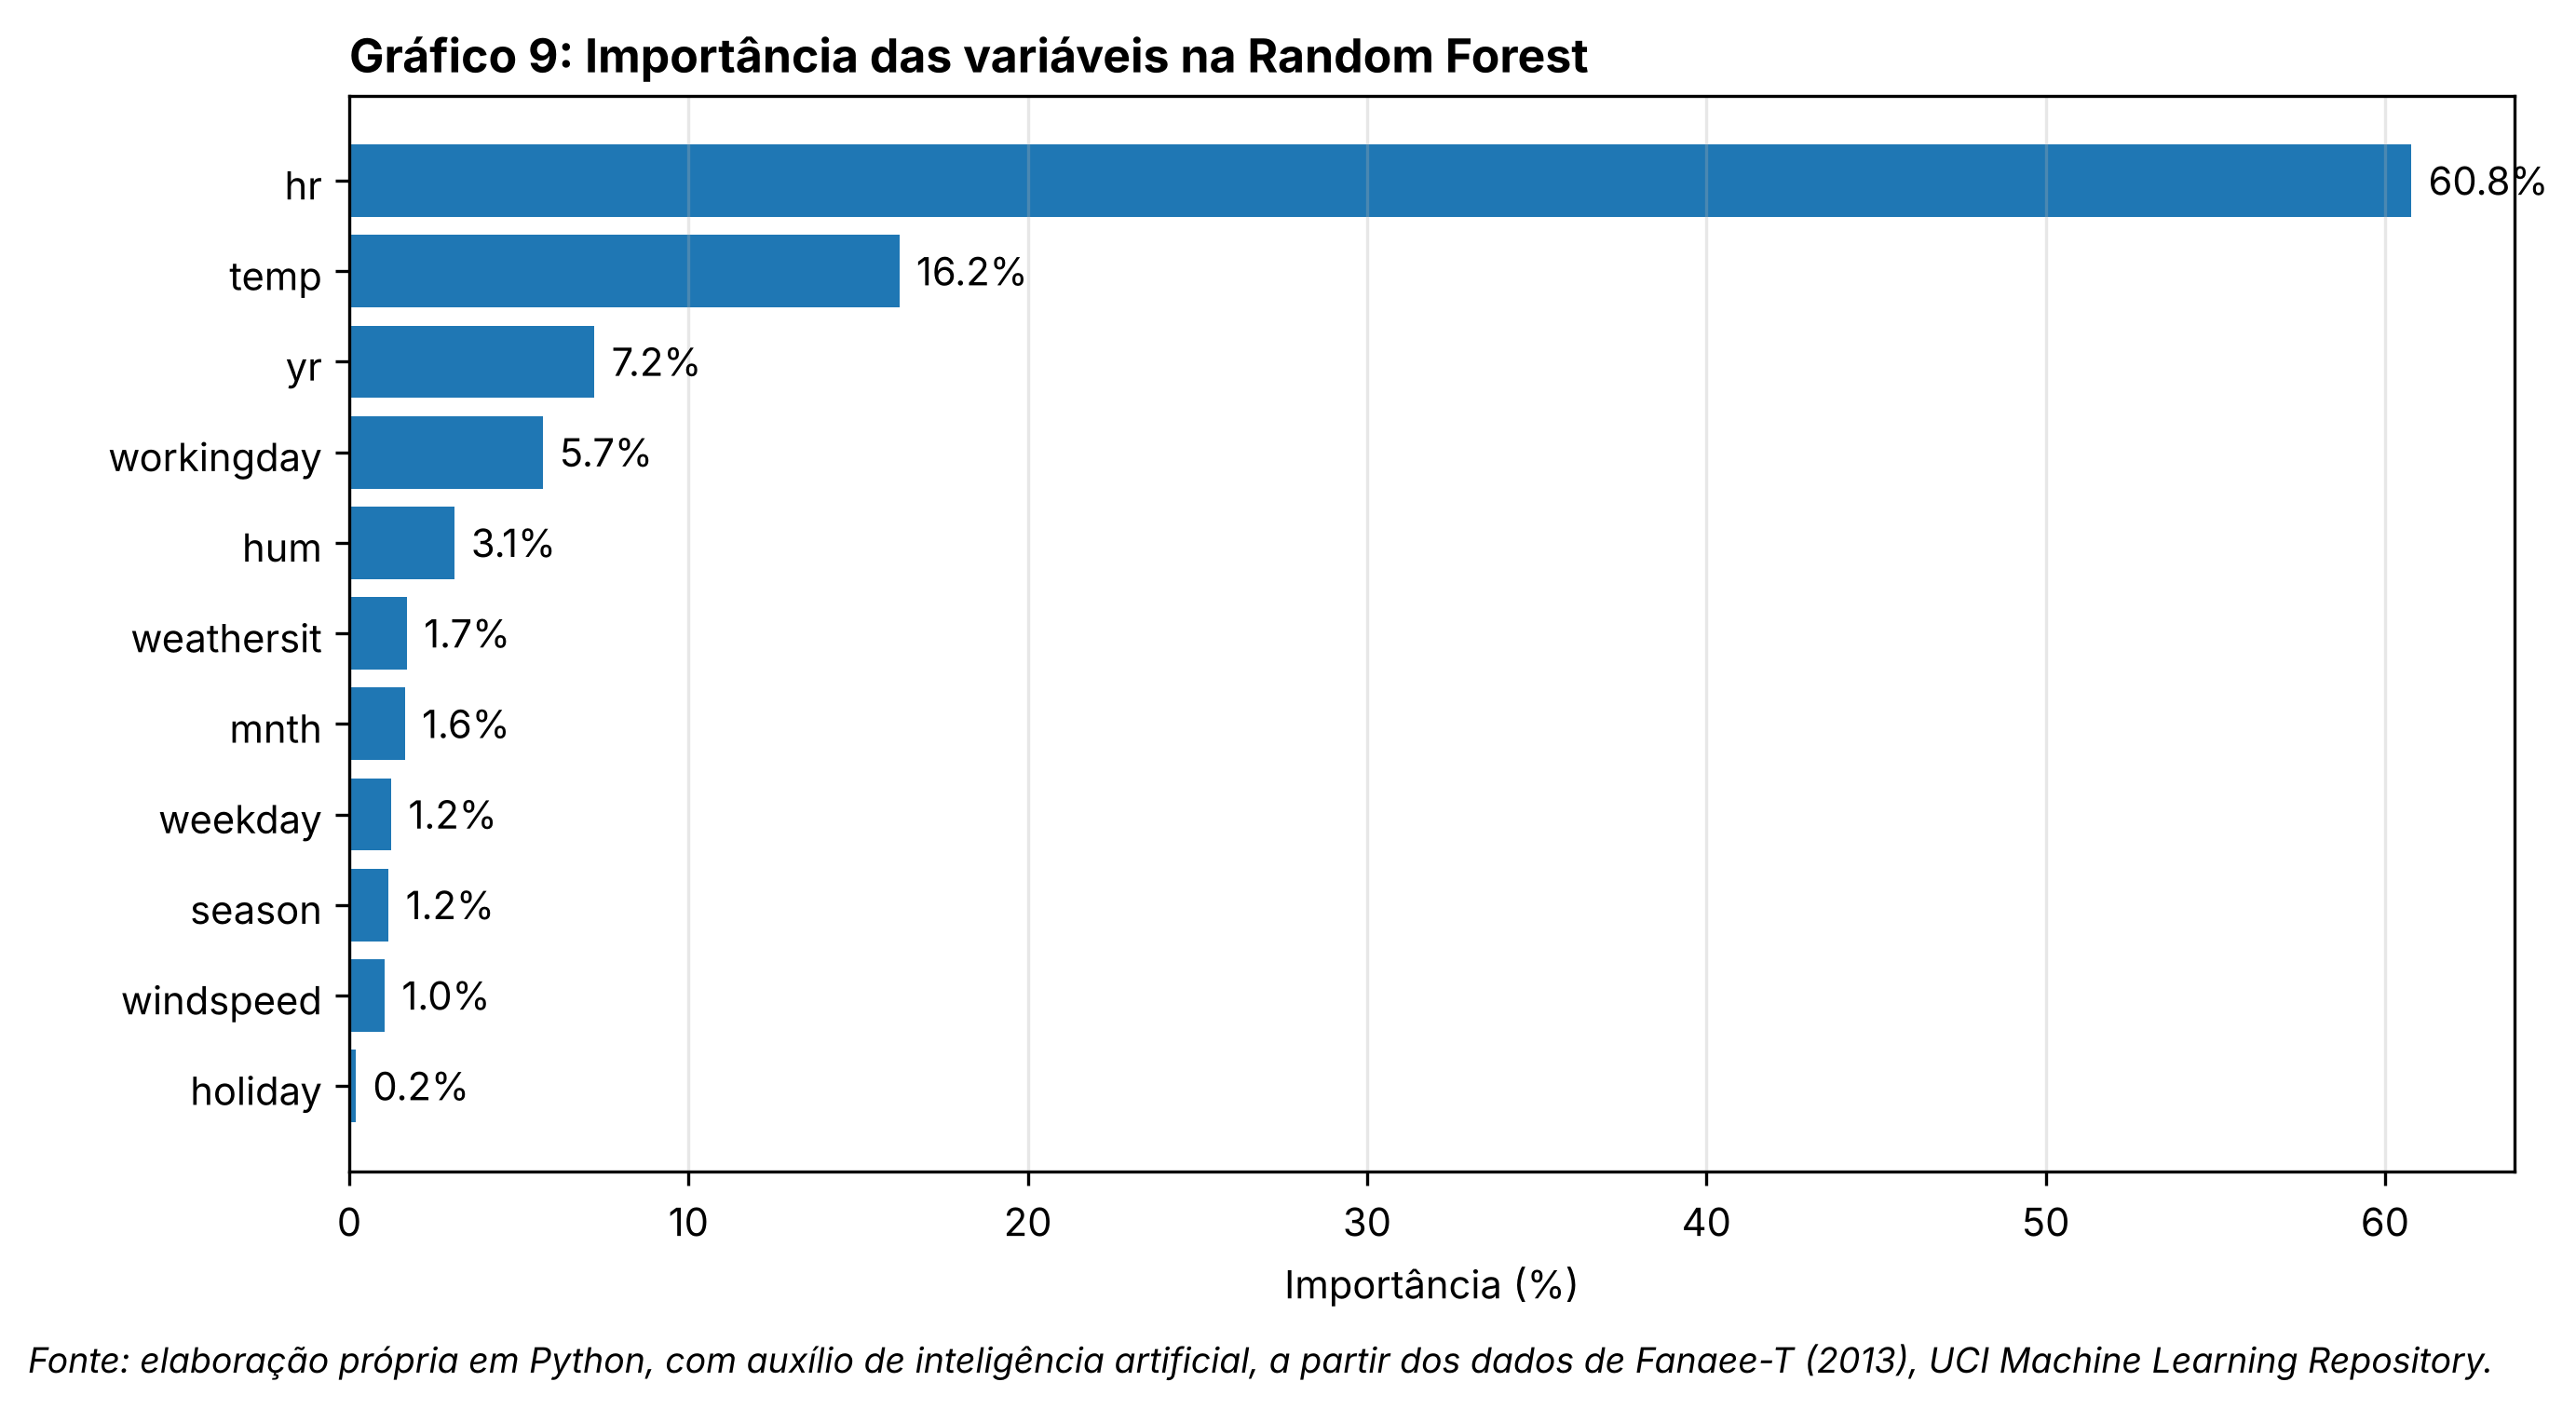
\includegraphics[width=0.80\linewidth,height=\textheight,keepaspectratio]{figuras/grafico_9.png}

}

\end{figure}%

\clearpage

\section{Limitações}\label{limitauxe7uxf5es}

O principal limite vem do próprio tipo de modelo: árvores e florestas
não preveem valores maiores do que os vistos no treino. Como a demanda
subiu de 2011 para 2012 e os únicos meses de outubro a dezembro vistos
no treino são os de 2011, a floresta ficou abaixo do valor real em 68\%
dos dias de outubro e 83\% dos de novembro de 2012. O mesmo efeito é
visível na árvore de profundidade 10 (Gráfico 7):
previsões abaixo do real em boa parte de outubro e novembro e acima dele
no fim de dezembro, quando a queda de demanda das festas leva o modelo a
prever mais do que ocorreu. Se o sistema continuasse crescendo, o modelo
teria de ser retreinado com frequência.

Os dados cobrem só dois anos de uma cidade, Washington, numa fase de
expansão do serviço, então os padrões podem não valer para outra cidade,
como o Recife. Eventos como o furacão Sandy não são previsíveis com
essas variáveis, e as 165 horas faltantes não foram preenchidas. Usamos
o clima observado em cada hora, e não a previsão do tempo, então o
desempenho real seria um pouco pior. Além disso, a profundidade da
árvore foi definida com um único período de validação, a floresta não
foi ajustada além das 200 árvores, e o teste cobre só um trimestre. Como
próximos passos, valeria incluir a demanda das horas anteriores, tratar
a tendência de crescimento separadamente, ajustar a floresta com
validação cruzada temporal (\emph{TimeSeriesSplit}), prever log(1 +
\texttt{cnt}) e comparar com \emph{gradient boosting}.

\section{Conclusão}\label{conclusuxe3o}

O objetivo era prever quantas bicicletas são alugadas por hora no
Capital Bikeshare a partir de calendário e clima. A base, aparentemente
sem problemas, tinha umidade zerada em um dia, sensação térmica travada
em outro, uma categoria de clima com 3 registros e 165 horas faltantes,
e cada caso foi tratado ou documentado. A exploração mostrou que a hora
do dia é o que mais muda a demanda (picos às 8h e entre 17h e 18h nos
dias úteis; uso concentrado entre 12h e 17h nos fins de semana), que se
aluga menos no inverno e mais no verão, que a demanda acompanha a
temperatura até cerca de 20--30 °C e depois cai, e que o uso cresceu
cerca de 63\% de 2011 para 2012.

Na modelagem, com divisão temporal, a floresta aleatória teve o melhor
resultado (MAE = 46,9; RMSE = 72,0; R² = 0,872), reduzindo o erro em
41\% frente ao \emph{baseline} e em 17\% frente à melhor árvore. As
variáveis mais usadas por ela (hora, temperatura, ano e dia útil) são as
mesmas que se destacaram na exploração. Assim, a árvore serve para
explicar as regras da demanda, mas a precisão exige a floresta. O
principal cuidado é que o modelo não acompanha o crescimento do sistema
e precisaria ser retreinado de tempos em tempos.

\section{Contribuições da equipe}\label{contribuiuxe7uxf5es-da-equipe}

O trabalho foi desenvolvido em conjunto: a equipe buscou se reunir ao
longo do projeto para discutir as escolhas de análise e modelagem, os
resultados obtidos e a interpretação de cada etapa, e as partes foram
divididas conforme descrito a seguir.

\begin{itemize}
\tightlist
\item
  \textbf{Raffael Marinho de Arruda Feitosa} ficou responsável pela
  elaboração do relatório, o que inclui a redação dos textos, a
  organização das seções e a apresentação dos resultados em tabelas e
  gráficos.
\item
  \textbf{Bruno Barbosa D'Antona} ficou responsável, principalmente,
  pela parte computacional: a escrita dos códigos de leitura, limpeza e
  modelagem dos dados e a geração dos gráficos usados no relatório.
\end{itemize}

\section*{Referências}\label{referuxeancias}
\addcontentsline{toc}{section}{Referências}

BREIMAN, L. Random forests. \emph{Machine Learning}, v. 45, n.~1,
p.~5-32, 2001.

FANAEE-T, H. \emph{Bike Sharing} {[}conjunto de dados{]}. UCI Machine
Learning Repository, 2013. DOI: 10.24432/C5W894.

FANAEE-T, H.; GAMA, J. Event labeling combining ensemble detectors and
background knowledge. \emph{Progress in Artificial Intelligence}, 2013.

PEDREGOSA, F. et al.~Scikit-learn: machine learning in Python.
\emph{Journal of Machine Learning Research}, v. 12, p.~2825-2830, 2011.

ROBERTS, D. R. et al.~Cross-validation strategies for data with
temporal, spatial, hierarchical, or phylogenetic structure.
\emph{Ecography}, v. 40, n.~8, p.~913-929, 2017.




\end{document}
